\part{Аналитическая геометрия}
\chapter{Метод координат}
\section{Величина направленного отрезка. Теорема Шаля. Декартова система
	координат на прямой.}
$\bullet$ \textit{\textbf{Отрезком} называется часть прямой, ограниченная двумя точками. Отрезок называется \textbf{направленным,} если указано, какая из граничных точек является начальной и какая
	конечной (Обозначения: $\overline{AB}$ – направленный отрезок; $| \overline{AB} |$ – длина направленного отрезка).} \\\\
$\bullet$ \textit{Отрезок называется \textbf{нулевым}, если его начальная и конечная точки совпадают.}\\\\
Длина нулевого направленного отрезка равна нулю.\\\\
$\bullet$ \textit{Прямая линия с указанным на ней направлением называется \textbf{осью}}.\\\\
$\bullet$ \textit{Пусть дана некоторая ось $\Delta$, и на ней расположен направленный отрезок $\overline{AB}$, \textbf{величиной} которого на оси $\Delta$ называется число, равное:}\begin{center}
	$AB = \begin{cases}
		|\overline{AB}|,\ \overline{AB} \uparrow \uparrow \Delta,\\
		-|\overline{AB}|,\ \overline{AB} \uparrow \downarrow \Delta;
	\end{cases}$
\end{center}
\textbf{\textit{Свойства величины направленного отрезка:}}\begin{enumerate}
	\item \textit{Величина $AB$ противоположна величине $BA$.}
	\item \textit{Длина $|\overline{AB}|$ равна модулю величин $AB$}.
\end{enumerate}
\newtheorem*{t1_1}{Теорема Шаля}\begin{t1_1}При любом расположении трех точек $A$, $B$ и $C$ на оси справедливо равенство $AB + BC = AC$.
\end{t1_1}
\begin{Proof}
	\begin{enumerate}
		\item Пусть точка $B$ лежит между точками $A$ и $C$, тогда направленные отрезки $\overline{AB}$, $\overline{BC}$ и $\overline{AC}$ сонаправлены. При этом $|\overline{AB}| + |\overline{BC}| = |\overline{AC}|$.
		\begin{enumerate}
			\item Если направляющие оси совпадают с направлениями отрезков, то $|\overline{AB}| = AB,\ |\overline{BC}| = BC,\  |\overline{AC}| = AC$. Следовательно, $AB + BC = AC$.
			\item Если направляющие оси не совпадают с направлениями отрезков, то $|\overline{AB}| = -AB,\ |\overline{BC}| = -BC,\  |\overline{AC}| = -AC$. Следовательно, $-AB + -BC = -AC\Rightarrow AB + BC = AC$.
		\end{enumerate}
		\item Если точка $C$ лежит между точками $A$ и $B$, то, по доказанному выше, $AC + CB = AB\Rightarrow AC = AB - CB = AB + BC$.
		\item Если точка $A$ лежит между точками $B$ и $C$, то $BA + AC = BC\Rightarrow AC = - BA + BC = AB + BC$.
	\end{enumerate}
	Теорема остается справедливой, даже если некоторые точки совпадают.
\end{Proof}\\\\
Пусть на прямой $\Delta$ дана точка $O$, заданы единица масштаба и определенное направление.\\\\
$\bullet$ \textit{Говорят, что на
	прямой $\Delta$ задана \textbf{декартовая система координат}. При этом ось $\Delta$ называется
	\textbf{координатной осью}, а точка $O$ – \textbf{началом координат}}.\\\\
Пусть точка $A$ --- некоторая фиксированная точка на прямой $\Delta$.\\\\
$\bullet$ \textit{\textbf{Координатой точки} $A$ называется число, равное
	величине $OA$ направленного отрезка $\overline{OA}$. Обозначение: $X_A$.} \\\\
Точки, расположенные по одну сторону от начала координат, имеют одинаковые по знаку координаты. Полуось, на которой все точки имеют положительные координаты, называют
положительной полуосью. Аналогично с отрицательной полуосью.
\newtheorem*{t1_2}{Теорема}\begin{t1_2} Для любых двух точек $A$ и $B$ на $\Delta$ выполняется: $AB = X_B - X_A$, $|\overline{AB}| = |X_B - X_A|$
\end{t1_2}\begin{Proof}
	Рассмотрим величину направленного отрезка $\overline{AB}$. Тогда, по теореме Шаля, $AB = AO + OB = OB-OA = X_B-X_A$
\end{Proof}\\\\
Пусть на оси $\Delta$ заданы 2 различные точки: $A$ с координатой $X_A$ и $B$ с координатой $X_B$.\\\\
$\bullet$ \textit{Говорят, что точка $C$ \textbf{делит} направленный отрезок $AB$ в отношении $\lambda$, если $\lambda = \dfrac{AC}{CB}$. При этом число $\lambda$ называется \textbf{простым отношением} трех точек $A, C, B$.}
\begin{enumerate}
	\item Если точка $C$ лежит между точками $A$ и $B$, то направляющие отрезки $AC$ и $CB$ сонаправлены. Следовательно, знак у них одинаковый и $\lambda>0$. При этом говорят, что точка $C$ делит направленный отрезок $AB$ внутренним образом.
	\item Если точка $C$ лежит вне отрезка $AB$, то говорят, что она делит отрезок $AB$ внешним образом. При этом отрезки $AC$ и $CB$ противоположно направлены (не сонаправлены) и, следовательно, $\lambda <0$.
	\item Если $\lambda = 0$, то $AC = 0$, следовательно, $|\overline{AC}| = 0$ и точки $A$ и $C$ совпадают.
	\item Если точка $C$ лежит за концом отрезка $AB$, то $\left |\dfrac{AC}{CB}\right | = \dfrac{|AC|}{|CB|} = \dfrac{|\overline{AC}|}{|\overline{CB}|} <1\Rightarrow \lambda < -1\ (|\overline{AC}| >  |\overline{BC}|)$.
	\item Если точка $C$ лежит перед началом отрезка $AB$, то $|\overline{AC}| < |\overline{BC}|$, тогда $-1 < \lambda < 0$.
\end{enumerate}
Заметим, что $\lambda \ne -1$, так как в этом случае $-1 = \frac{AC}{CB}$. Следовательно, $AC = -CB\Rightarrow AC = CB\Rightarrow A$ и $B$ совпадают, что противоречит выбору $A$ и $B$.
\newtheorem*{t1_3}{Теорема}\begin{t1_3}
	Координата точки $C$, делящей направленный отрезок $AB$ в отношении $\lambda$ равна $$X_C = \dfrac{X_A + \lambda X_B}{1+\lambda}$$
\end{t1_3}\begin{Proof}
	Из определения деления отрезка в данном отношении следует:\\\\ $\lambda = \dfrac{AC}{CB} = \dfrac{X_C - X_A}{X_B-X_C}\Rightarrow (X_B - X_C)\cdot \lambda = X_C - X_A\Rightarrow \lambda X_B + X_A = X_C + \lambda X_C = X_C(1 + \lambda)\Rightarrow \\\\X_C = \dfrac{X_A+\lambda X_B}{1+ \lambda}$
\end{Proof}










\section{Декартова прямоугольная система координат на плоскости, в пространстве (ДПСК).}
$\bullet$ \textit{\textbf{Декартовой прямоугольной системой координат на плоскости} называются две взаимно перпендикулярные координатные оси с общим началом координат. Ось $Ox$ называется осью \textbf{абсцисс}, $Oy$ --- осью \textbf{ординат}. \\\\$\bullet$ Система координат называется \textbf{правой}, если кратчайший поворот от оси $X$ к оси $Y$ против часовой стрелки, иначе \textbf{левой}.}\\
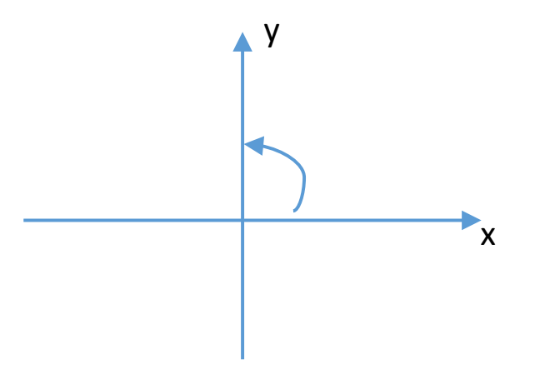
\includegraphics[scale=0.3]{images/rdpsk.png} \qquad\qquad\qquad\qquad\qquad 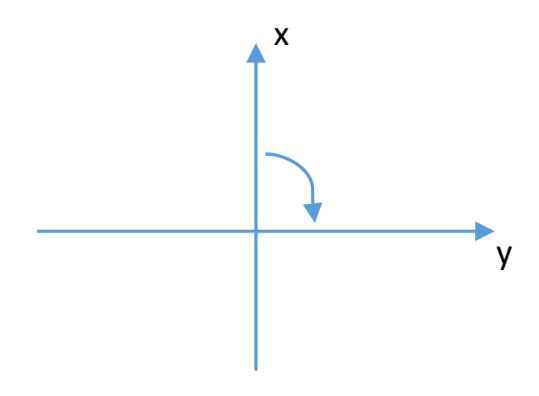
\includegraphics[scale=0.3]{images/ldpsk.png}\par
\quadПравая ДПСК\qquad\qquad\qquad\qquad\qquad\qquad\qquad\qquad\qquadЛевая ДПСК\\\\
Пусть $M$ --- некоторая точка плоскости, $M_x$ и $M_y$ --- проекции на оси $Ox$ и $Oy$ соответственно.\\\\
$\bullet$ \textit{\textbf{Декартовыми прямоугольными координатами} точки $M(X_M, Y_M)$ называются величины направленных отрезков $\overline{OM_x}$ и $\overline{OM_y}$ на координатных осях, то есть $X_M = OM_x,\ Y_M = OM_y$.}\\\\
Пусть $A(X_A, Y_A)$ и $B(X_B, Y_B)$ --- две различные точки на плоскости.
\newtheorem*{t2_1}{Теорема}\begin{t2_1}Длина направленного отрезка $\overline{AB}$ равна:
	$$|\overline{AB}| = \sqrt{(X_A - X_B)^2 + (Y_A - Y_B)^2}$$\end{t2_1}
\begin{Proof}
	Построим проекции точек $A$ и $B$ на координатные оси. Обозначим через $C$ точку пересечения проекций.\begin{center}
		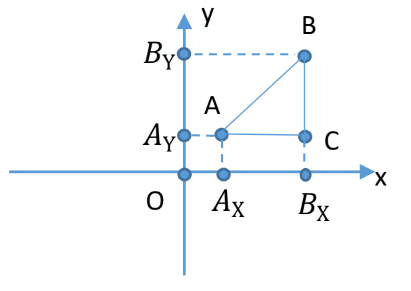
\includegraphics[scale=0.4]{images/t2_1dpsk.png}
	\end{center}
	По теореме Пифагора $|AB|^2 = |AC|^2 + |BC|^2$. Тогда $|\overline{AB}| = \sqrt{|\overline{A_xB_x}|^2 + |\overline{A_yB_y}|^2} =\\ =\sqrt{(X_A - X_B)^2 + (Y_A - Y_B)^2}$.\\\\
	Рассмотрим случай, когда отрезок $AB$ параллелен $Ox$ (или $AB$ параллелен $Oy$). Тогда $Y_A = Y_B$ и $\sqrt{(X_A - X_B)^2 + \underbrace{(Y_A - Y_B)^2}_{=0}} = |X_A - X_B| = |\overline{AB}| = |\overline{A_xB_x}|$.
\end{Proof}\\\\
Проведем через точки $A$ и $B$ некоторую ось. Тогда имеет смысл понятие «деление отрезка в данном отношении».
\newtheorem*{t2_2}{Теорема}\begin{t2_2}Координаты точки $C$, делящей $\overline{AB}$ в отношении $\lambda$, равны: $$X_C = \dfrac{X_A + \lambda X_B}{1+\lambda},\ Y_C = \dfrac{Y_A + \lambda Y_B}{1+\lambda}$$\end{t2_2}\begin{Proof}
	Построим проекции точек $A$, $B$ и $C$ на ось $Ox$. Заметим, что при любом расположении точки $C$ точка $C_x$ будет иметь такой же характер расположения, как и точка $C$ (если $C$ лежит между $A$ и $B$, то и $C_x$ будет лежать между $A_x$ и $B_x$). Следовательно, $\dfrac{|\overline{AC}|}{|\overline{CB}|}$ и $\dfrac{\overline{A_xC_x}}{\overline{C_xB_x}}$ имеют один знак.\\
	По теореме Фалеса длина $\dfrac{|\overline{A_xC_x}|}{|\overline{C_xB_x}|} = \dfrac{|\overline{AC}|}{|\overline{CB}|}\Rightarrow\left | \dfrac{A_xC_x}{C_xB_x}  \right | = \left | \dfrac{AC}{CB}  \right |$. Следовательно, $\dfrac{A_xC_x}{C_xB_x} = \dfrac{AC}{CB} = \lambda$ и точка $C_x$ делит направленный отрезок $\overline{A_xB_x}$ также в отношении $\lambda$. Следовательно, $X_C = \dfrac{X_A + \lambda X_B}{1+\lambda}$. \\Для ординаты точки $C$ равенство доказывается аналогично при рассмотрении случая, когда прямая $AB$ параллельна одной из осей.
\end{Proof}\\\\
$\bullet$ \textit{\textbf{ДПСК в пространстве} образуют три взаимно перпендикулярные координатные оси с общим началом координат.
	Треться ось $Oz$ называется осью \textbf{аппликатой}.\\\\$\bullet$
	Система координат называется \textbf{правой}, если, глядя со стороны направления $Oz$,
	кратчайший поворот от оси $Ox$ к оси $Oy$ осуществляется против часовой стрелки, иначе --- \textbf{левой}.}\\\\
Пусть $A(X_A,Y_A,Z_A)$ и $B(X_B,Y_B,Z_B)$ --- две различные точки пространства. Тогда\begin{enumerate}
	\item $|\overline{AB}| = \sqrt{(X_A - X_B)^2 + (Y_A - Y_B)^2 + (Z_A - Z_B)^2}$
	\item Если $C$ делит $\overline{AB}$ в отношении $\lambda$, то
	$$X_C = \dfrac{X_A + \lambda X_B}{1+\lambda},\ Y_C = \dfrac{Y_A + \lambda Y_B}{1+\lambda},\ Z_C = \dfrac{Z_A + \lambda Z_B}{1+\lambda}.$$
\end{enumerate}






\section{Полярные, цилиндрические и сферические координаты. Общая декартова система координат.}
$\bullet$ \textit{\textbf{Полярную систему координат} образуют точка, выходящий из неё луч и единичный отрезок. При этом точка $O$ называется \textbf{полюсом}, а луч $Ox$ --- полярной осью.}\begin{center}
	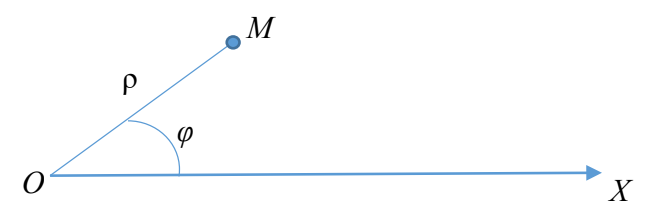
\includegraphics[scale=0.4]{images/polar.png}
\end{center}
Пусть $M$ --- произвольная точка плоскости.\\\\
$\bullet$ \textit{\textbf{Полярными координатами точки} $M$ называются два числа $\rho, \varphi$, где $\rho$ --- длина $OM$ ($\rho = |\overline{OM}|$), а угол $\varphi$ равен углу, на который необходимо повернуть полярную ось вокруг точки $O$ против часовой стрелки до совмещения ее с отрезком $OM$.}\\\\
$\bullet$ \textit{Число $\rho$ называется \textbf{полярным радиусом} точки. Число $\varphi$ --- \textbf{полярным углом} точки.}\\\\
Заметим, что $\rho \geqslant 0$, а $\varphi$ определён с точностью до $2\pi k$, где $k\in \mathbb{Z}$. Точка $O$ имеет $\rho = 0$, а $\varphi$ для неё не определён (ему можно приписать любое направление).\\
Значение $\varphi$, принадлежащее $[0;2\pi)$, называется главным значением $\varphi$.\\
Полярной осью называют точку и выходящий из неё луч.\\\\
Покажем связь между декартовой и полярной системами координат.\\
Расположим ДПСК и ПСК следующим образом: полюс поместим в начало координат, а полярную ось совместим с положительной полуосью $Ox$. Расположенные таким образом ДПСК и ПСК называют \textbf{соответствующими друг другу}.\begin{center}
	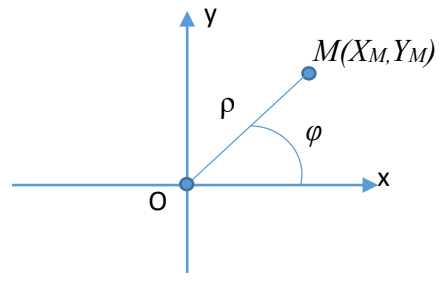
\includegraphics[scale=0.4]{images/d_psk.png}
\end{center}
Пусть $M$ произвольная точка плоскости. Тогда полярные координаты точки $M$ равны: \\$X_M = OM_x = |OM|\cdot cos\varphi = \rho\cdot cos\varphi,$\\
$Y_M = OM_y = |OM|\cdot sin\varphi = \rho\cdot sin\varphi$, где $\rho = \sqrt{X_M^2 + Y_M^2}$, а угол $\varphi$ можно найти, решив следующую систему:$\begin{cases}
	cos\varphi = \dfrac{X_M}{\rho} = \dfrac{X_M}{\sqrt{X_M^2 + Y_M^2}},\\\\
	sin\varphi = \dfrac{Y_M}{\rho} = \dfrac{Y_M}{\sqrt{X_M^2 + Y_M^2}};
\end{cases}$\\\\
Цилиндрическая и сферическая системы координат в пространстве вводятся следующим образом: в пространстве зафиксируем некоторую плоскость П. Построим на ней полярную систему координат, а так же координатную ось $Oz$ с началом в точке $O$ и перпендикулярную плоскости П.\begin{center}
	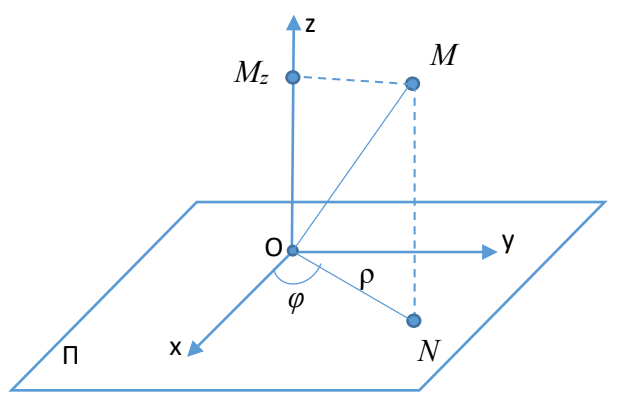
\includegraphics[scale=0.3]{images/pcsk.png}
\end{center}
И пусть точка $M$ --- произвольная точка пространства, а отрезок $MN$ --- её проекция на плоскость П.\\\\
$\bullet$ \textit{\textbf{Цилиндрическими координатами точки} $M$ называются числа $\rho, \varphi, z$, где $\rho$ и $\varphi$ --- полярные координаты точки $N$ относительно построенной полярной системы координат, а $z$ --- величина направленного отрезка $\overline{OM_z}$ ($z = OM_z$)}.\\\\
$\bullet$ \textit{\textbf{Сферическими координатами точки} $M$ называются три числа $\rho, \varphi, \Theta$, где $\rho$ --- длина отрезка $|\overline{OM}|$, $\varphi$ --- полярный радиус точки $N$ относительно построенной полярной системы координат, а $\Theta$ --- угол между направленным отрезком $\overline{OM}$ и осью $Oz$.}\\\\
Из определений следует, что $\rho\geqslant0$ и для цилиндрических, и для сферических координат, $\Theta\in [0;\pi]$, а $\varphi$ определён с точностью до $2\pi n, n\in \mathbb{Z}$.\\\\
Построим в пространстве ДПСК следующим образом: начало координат совпадает с точкой $O$, ось $Oz$ совместим с построенной ранее осью $Oz$, а положительное направление оси $Ox$ --- с полярной осью. \begin{center}
	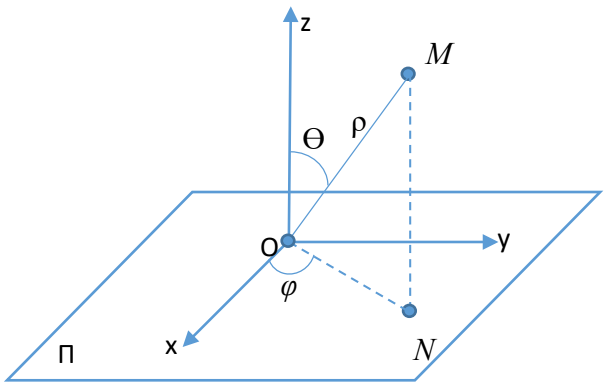
\includegraphics[scale=0.3]{images/pcsk_2.png}
\end{center}
Тогда точка $M$ имеет следующие координаты в системах:\begin{center}
	цилиндрическая: $\begin{cases}
		X_M = \rho\cdot cos\varphi,\\
		Y_M = \rho\cdot sin\varphi,\\
		Z_M = z;
	\end{cases}$ сферическая: $\begin{cases}
		X_M = \rho\cdot cos\varphi\cdot sin\Theta,\\
		Y_M = \rho\cdot sin\varphi\cdot sin\Theta,\\
		Z_M = \rho\cdot cos\Theta.
	\end{cases}$
\end{center}
$\bullet$ \textit{\textbf{Общую декартову систему координат (Аффинную систему координат)} на плоскости образуют две пересекающие координатные оси с общим началом координат.}\\\\
Пусть точка $M$ --- произвольная точка плоскости. Построим через точку $M$ прямые, параллельные координатным осям.\begin{center}
	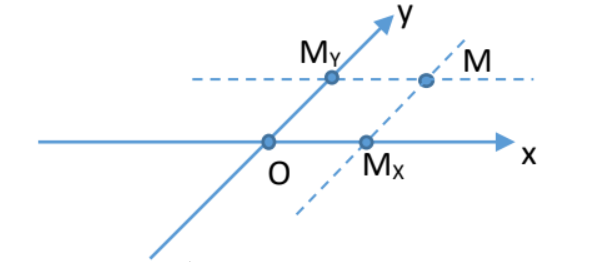
\includegraphics[scale=0.3]{images/odsk.png}
\end{center}
$\bullet$ \textit{\textbf{Общими декартовыми координатами точки} $M$ называются величины направленных отрезков $\overline{OM_x}$ и $\overline{OM_y}$}.











\chapter{Векторы}
\section{Понятие вектора. Линейные операции над векторами.}
$\bullet$ \textit{\textbf{Вектором} называется множество всех одинаково направленных отрезков равной длины. Обозначение: $a,b,c$ или $\vec{a}, \vec{b}, \vec{c}$.}\\\\
Пусть $\overline{AB}$ --- направленный отрезок. Тогда существует единственный вектор, которому принадлежит этот отрезок. То есть любой направленный отрезок $\overline{AB}$ однозначно определяет вектор, который обозначается как $\overrightarrow{AB}$.\\\\
Пусть заданы вектор $\vec{a}$ и некоторая точка $A$. Тогда существует единственная точка $B$, такая, что $a = \overrightarrow{AB}$.\\\\
$\bullet$ \textit{Операция построения такой точки $B$ называется \textbf{откладыванием} вектора $\vec{a}$ от точки $A$.\\\\$\bullet$
	\textbf{Длиной вектора} $\vec{a}$ называется длина любого из направленных отрезков среди его образующих. Обозначение: $|\vec{a}|$.}\\\\$\bullet$
\textit{Вектор длины 0 называется \textbf{нулевым}. Обозначение: $\vec{0}$. Вектор длины 1 называется \textbf{единичным} или \textbf{ортом}.}\\\\$\bullet$
\textit{Векторы называются \textbf{коллинеарными}, если образующие их отрезки параллельны
	некоторой прямой.\\\\$\bullet$
	Векторы называются \textbf{компланарными}, если образующие их отрезки параллельны
	некоторой плоскости.}\\\\
Заметим, что нулевой вектор и коллинеарен любому вектору, и компланарен любым двум другим
векторам.\\\\
Пусть $a$ и $b$ --- 2 ненулевых вектора, отложенных от некоторой точки $O$. То есть найдём такие точки $A$, и $B$, что $a = \overrightarrow{OA}, b = \overrightarrow{OB}$.\\\\
$\bullet$ \textit{\textbf{Углом между векторами} $a$ и $b$ называертся угол между направленными отрезками $\overline{OA}$ и $\overline{OB}$.}
\begin{center}
	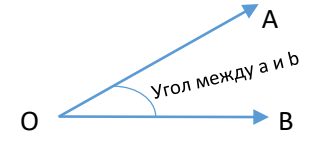
\includegraphics[scale=0.4]{images/cornAB.png}
\end{center}
Из определения следует, что угол между двумя векторами $\in [0; \pi]$.\\\\
\textbf{\textit{Линейные операции над векторами:}}\begin{itemize}
	\item сложение;
	\item умножение на число.
\end{itemize}
Пусть $a$ и $b$ --- два вектора. Возьмем некоторую точку $O$ и отложим от нее вектор $a = \overrightarrow{OA}$. Затем от точки $A$ отложим вектор $b = \overrightarrow{AB}$.
\begin{center}
	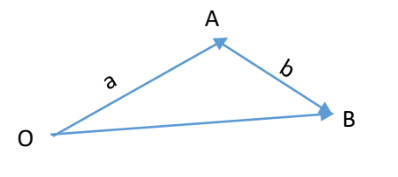
\includegraphics[scale=0.4]{images/vectriangle.png}
\end{center}
$\bullet$ \textit{\textbf{Суммой векторов} $a$ и $b$ будет называться вектор $\overrightarrow{OB}$. Обозначение: $a+b$.}\\\\
$\bullet$ \textit{\textbf{Произведением вектора} $a$ на действительное число $A$ называется вектор, длина которого равна $|A|\cdot |a|$, а направление совпадает с направлением вектора $a$, если $A>0$, и противоположно направлению вектора $a$, если $A<0$. Обозначение: $A\cdot a$. }\\\\
\textbf{\textit{Свойства линейных операций:}}\begin{enumerate}
	\item $a+b = b+a$.\begin{Proof}
		Пусть $a = \overrightarrow{OA},\ b=\overrightarrow{AB}$. На направленных отрезках $\overline{OA}$ и $\overline{AB}$ построим параллелограмм $OABC$.\begin{center}
			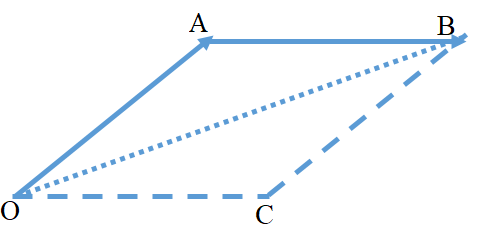
\includegraphics[scale=0.65]{images/vec_sum.png}
		\end{center}
		Заметим, что векторы $\overrightarrow{CB}$ и $\overrightarrow{OA}$ сонаправлены и $|\overline{CB}| = |\overline{OA}|$. Следовательно, $\overrightarrow{CB} = \overrightarrow{OA} = a$. Путем аналогичных рассуждений получим $\overrightarrow{OC} = \overrightarrow{AB} = b$.\\
		По определению суммы векторов, вектор $\overrightarrow{OB}$ можно, с одной стороны, рассматривать как сумму векторов $\overrightarrow{OA} + \overrightarrow{AB}$, а с другой стороны, как сумму $\overrightarrow{OC} + \overrightarrow{CB}$. Следовательно, $\overrightarrow{OB} = \begin{cases}
			\overrightarrow{OA} + \overrightarrow{AB} = a + b,\\
			\overrightarrow{OC} + \overrightarrow{CB} = \overrightarrow{AB} + \overrightarrow{OA} = b + a;
		\end{cases}\Rightarrow a + b = b + a.$			
	\end{Proof}
	\item $(a+b) + c = a + (b+c)$.
	\item $\vec{a} + \vec{0} = \vec{a},\quad \forall \vec{a}$.
	\item $\alpha(a+b) = \alpha a + \alpha b$,\\
	$(\alpha + \beta) a = \alpha a + \beta a$,\\
	$\alpha(\beta a) = (\alpha\beta) a$, где $a,b$ --- векторы, $\alpha, \beta$ --- числа.
\end{enumerate}
$\bullet$ \textit{Вектор $b$ называется \textbf{противоположным} вектору $a$, если его длина совпадает с длиной вектора $a$, а направление противоположно.}\\\\
Из определения следует, что\begin{enumerate}
	\item $-1\cdot a = -a$, где вектор $(-a)$ --- противоположный вектору $a$;
	\item $1\cdot a = a$.
\end{enumerate}
$\bullet$ \textit{\textbf{Разностью векторов} $a$ и $b$ называется вектор, прибавив который к вектору $b$, получим вектор $a$, то есть вектор $c = a-b$, где $c+b = a$.}\\\\
\textbf{Правило вычитания:} \textit{Чтобы из вектора $a$ вычесть вектор $b$, необходимо к вектору $a$ прибавить вектор, противоположный вектору $b$, то есть $a-b = a + (-b)$.}\\\begin{Proof}
	$(a+(-b)) + b = a + (b + (-b)) = a + \vec{0} = a$.
\end{Proof}



\section{Координаты вектора.}
Пусть $a_1,\dots,a_k$ --- произвольная система векторов. $\alpha_1,\dots,\alpha_k$ --- некоторые действительные числа.\\\\
$\bullet$ \textit{Вектор $\alpha_1 a_1 + \ldots + \alpha_k a_k$ называется линейной комбинацией векторов $a_1,\dots,a_k$ с коэффициентами $\alpha_1,\dots,\alpha_k$.}\\\\
Если вектор представлен в виде линейной комбинации системы векторов (то есть $b = \alpha_1 a_1 + \ldots + \alpha_k a_k$), то говорят, что данный вектор разложим по этим векторам системы.\\\\
$\bullet$ \textit{\textbf{Базисом на прямой} называется любой ненулевой вектор, параллельный этой прямой.}\\\\
$\bullet$ \textit{\textbf{Базисом на плоскости} называется упорядоченная пара неколлинеарных векторов.}\\\\
$\bullet$ \textit{\textbf{Базисом в пространстве} называется упорядоченная тройка некомпланарных векторов.}\\\\
Нулевой вектор не может быть элементом базиса.
\newtheorem*{th2_2_1}{Теорема}\begin{th2_2_1}\end{th2_2_1}
\begin{enumerate}
	\item \textit{Любой вектор, параллельный прямой, может быть единственным образом разложен по базису этой прямой.}
	\item \textit{Любой вектор, параллельный плоскости, может быть единственным образом разложен по базису на этой плоскости.}
	\item \textit{Любой вектор в пространстве может быть единственным образом по базису в пространстве.}
\end{enumerate}
\begin{Proof}
	Покажем существование разложения для каждого из пунктов.\begin{enumerate}
		\item Пусть $\Delta$ --- некоторая прямая, $a$ --- базис на ней, $b$ --- вектор, параллельный $\Delta$. Тогда $a \parallel b\Rightarrow a$ и $b$ коллинеарны.\\\\
		Пусть $e_a,\ e_b$ --- единичные векторы, параллельные векторам $a$ и $b$ соответственно. Так как $e_a = \dfrac{1}{|a|}a,\ e_b = \dfrac{1}{|b|}b$ и $a$ и $b$ коллинеарны, то и $e_a$ и $e_b$ также коллинеарны. Следовательно, они либо противоположные, либо равные.\\\\
		Если они равные, то $e_a = e_b \Rightarrow\dfrac{1}{|a|}a = \dfrac{1}{|b|}b\Rightarrow b = \dfrac{|b|}{|a|}a = $[замена $\dfrac{|b|}{|a|}$ на $l$]$ = la$\\\\
		Если они противоположные, то $e_a = -e_b \Rightarrow\dfrac{1}{|a|}a = -\dfrac{1}{|b|}b\Rightarrow b = -\dfrac{|b|}{|a|}a = $[замена $-\dfrac{|b|}{|a|}$ на $l$]$ = la\Rightarrow$ вектор $b$ разложим по базису $a$.
		\item Пусть П --- некоторая плоскость, $a_1$ и $a_2$ --- базис на плоскости, $b$ $\parallel$ П $\Rightarrow a_1,\ a_2,\ b$ --- компланарны. Отложим векторы базиса от некоторой точки О на плоскости П, то есть $a_1 = \overrightarrow{OA_1}, a_2 = \overrightarrow{OA_2}, b = \overrightarrow{OB}$.
		\begin{center}
			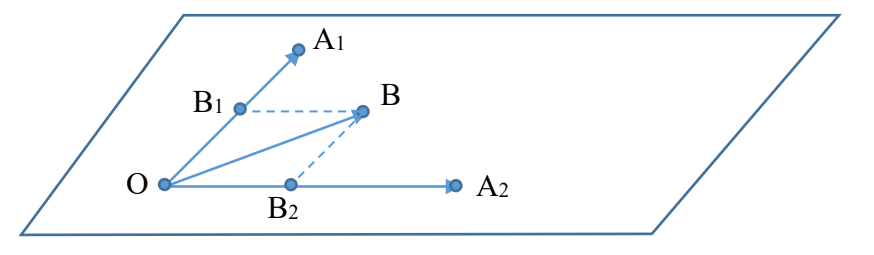
\includegraphics[scale=0.5]{images/pl_in_2_2.png}
		\end{center}
		Построим прямую, проходящую через точку $B$, параллельную $OA_2$. Пусть $B_1$ --- точка пересечения построенной прямой и прямой $OA_1$. Аналогично на $OA_2$ построим точку $B_2$.\\\\
		По определению суммы векторов $b = \overrightarrow{OB} = \overrightarrow{OB_1} + \overrightarrow{OB_2}.$ Тогда $OB_1 \parallel OA_1$, а ненулевой вектор $\overrightarrow{OA_1}$ является на этой прямой базисом. Следовательно, по доказанному выше в пункте 1, $\overrightarrow{OB_1} = l_1 \cdot \overrightarrow{OA_1} = l_1\cdot a_1$. По аналогичным рассуждениям получим $\overrightarrow{OB_2} = l_2\cdot a_2\Rightarrow b = l_1\cdot a_1 + l_2 \cdot a_2$.
		\item Доказательство данного пункта проводится по аналогичной схеме с пунктом 2. Покажем единственность: рассмотрим самый сложный вариант, в пространстве. На плоскости и прямой доказательства будут аналогичными.\\\\
		Пусть $a_1$, $a_2$, $a_3$ --- базис в пространстве, а $b$ --- некоторый вектор пространства. И пусть существуют 2 различных разложения:
		$\begin{cases}
			b = l_1 a_1 = l_2 a_2 + l_3 a_3,\\
			b = \beta_1 a_1 + \beta_2 a_2 + \beta_3 a _3;
		\end{cases}\Rightarrow$ [вычтем из первого второе] $\Rightarrow 0 = (l_1 - \beta_1) a_1 + (l_2 - \beta_2) a_2 + (l_3 - \beta_3) a_3$.\\
		Пусть $l_i - \beta_i\ne 0\Rightarrow a_1 = -\dfrac{l_2 - \beta_2}{l_1 - \beta_1}a_2 -\dfrac{l_3 - \beta_3}{l_1 - \beta_1}a_3\Rightarrow a_1,\ a_2,\ a_3$ --- компланарные, что является противоречием с тем, что базис в пространстве --- это 3 некомпланарных вектора $\Rightarrow l_i - \beta_i = 0\Rightarrow$ два разложения совпадают.
\end{enumerate}\end{Proof}\\
Пусть $a$ --- некоторый вектор в пространстве. $e_1$, $e_2$, $e_3$ --- некоторый базис в пространстве. По теореме выше вектор $a$ единственным образом представим в виде $l_1 e_1 + l_2 e_2 + l_3 e_3$.\\\\
$\bullet$ \textit{Коэффициенты разложения вектора $a$ по базису $e_1, e_2, e_3$ называются \textbf{координатами вектора $a$ в базисе $e_1, e_2, e_3$}. Обозначение: $a(l_1, l_2, l_3)$.}
\newtheorem*{th2_2_2}{Теорема}\begin{th2_2_2}
	При умножении вектора на число все его координаты умножаются на это число. При
	сложении векторов их соответствующие координаты складываются.
\end{th2_2_2}\begin{Proof}
	Пусть $a, b$ --- произвольные векторы, $e_1, e_2, e_3$ --- базис. $(l_1, l_2, l_3)$ и $(\beta_1, \beta_2, \beta_3)$ --- координаты векторов $a$ и $b$ в базисе $e_1, e_2, e_3$ соответственно. Тогда\\
	$l\cdot a = l\cdot(l_1 e_1 + l_2 e_2 + l_3 e_3) = l\cdot l_1 e_1 + l\cdot l_2 e_2 + l\cdot l_3 e_3$;\\
	$a+b = (l_1 e_1 + l_2 e_2 + l_3 e_3) + (\beta_1 e_1 + \beta_2 e_2 + \beta_3 e_3) = (l_1 + \beta_1) e_1 + (l_2 + \beta_2) e_2 + (l_3 + \beta_3) e_3$.\\
	Получили векторы с координатами $la(l\cdot l_1, l\cdot l_2, l\cdot l_3),\ a+b(l_1 + \beta_1, l_2 + \beta_2, l_3 + \beta_3)$.
\end{Proof}
\newtheorem*{cor2_2}{Следствие (критерий коллинеарности векторов)}\begin{cor2_2}Два ненулевых вектора $a$ и $b$ коллинеарны $\Longleftrightarrow$ их координаты пропорциональны.
\end{cor2_2}\begin{Proof}
	$\Rightarrow)$ Пусть $a(l_1, l_2, l_3), b(\beta_1, \beta_2, \beta_3)$ --- 2 ненулевых коллинеарных вектора $\Rightarrow$ вектор 
	$a$ является
	базисом на прямой $\Rightarrow$ $b$ представим в виде: $b = la \Rightarrow b$ имеет координаты $(l\cdot l_1, l\cdot l_2, l\cdot l_3)\Rightarrow$
	координаты пропорциональны.\\
	$\Leftarrow)$ Пусть координаты пропорциональны: $l\cdot l_i = \beta_i \Rightarrow b = \beta_1e_1 + \beta_2e_2 + \beta_3 e_3 = l\cdot l_1 e_1 + l\cdot l_2 e_2 + l\cdot l_3 e_3 =
	l\cdot(l_1e_1 + l_2e_2 + l_3e_3) = la \Rightarrow$ вектор $a$ либо $\uparrow \uparrow b$, либо $\uparrow\downarrow b$ $\Rightarrow a$ коллинеарен $b$.
\end{Proof}


\section{Декартовы координаты вектора.}
$\bullet$ \textit{Рассмотрим ДПСК $Oxyz$, и пусть $i, j, k$ --- единичные векторы, сонаправленные с осями $Ox, Oy, Oz$. Такие векторы называют \textbf{направляющими ортами} осей координат.}\\\\
$\bullet$ \textit{Векторы $i, j, k$ некомпланарны, следовательно, они образуют базис в пространстве. Данный базис является \textbf{ортонормированным базисом}.}\\\\
Пусть $a$ --- произвольный вектор пространства. Тогда по первой теореме из предыдущего параграфа $a = x\cdot i + y\cdot j + z\cdot k$, где $(x, y, z)$ --- декартовы координаты вектора $a$. То есть декартовы координаты вектора --- это коэффициенты при разложении этого вектора по ортонормированному базису.\\\\
Рассмотрим некоторый вектор $a$ и некоторую ось $\Delta$. Отложим вектор $a$ от точки $A$ и пусть $a = \overrightarrow{AB}$. Построим проекции $A$ и $B$ на ось $\Delta$ и пусть это будут точки $A_1$ и $B_1$.\\\\
$\bullet$ \textit{Полученный в результате направленный отрезок $\overline{A_1B_1}$ определяет вектор $\overrightarrow{A_1B_1}$, который называется \textbf{проекцией} вектора $a$ на ось $\Delta$.}\\\\
$\bullet$ \textit{Величина направленного отрезка $\overline{A_1B_1}$ называется \textbf{величиной проекции} вектора $a$ на ось $\Delta$. Обозначение: $\text{ПР}_\Delta a$}\\\\
\textbf{\textit{Свойства величин проекции вектора на ось:}}\begin{enumerate}
	\item $\text{ПР}_\Delta a = |a|\cdot cos\varphi$, где $\varphi$ --- угод между вектором $a$ и осью $\Delta$.
	\begin{Proof}
		Отложим от некоторой точки $O$ на оси $\Delta$ вектор $a$ (то есть $a = \overrightarrow{OA}$). $A_1$ --- проекция точки $A$. Тогда $\text{ПР}_\Delta a = OA_1$.\begin{center}
			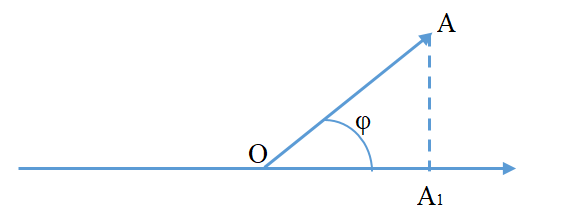
\includegraphics[scale=0.5]{images/corn2_3.png}
		\end{center}
		Если угол $\varphi$ острый, то $\text{ПР}_\Delta a = |\overline{OA_1}|\Rightarrow \text{ПР}_\Delta a = |\overline{OA}|\cdot cos(\varphi) = |a|\cdot cos(\varphi)$.\\\\
		Если угол $\varphi$ тупой, то $\text{ПР}_\Delta a = -|\overline{OA_1}| = -|\overline{OA}|\cdot cos(\pi - \varphi) = |\overline{OA}|\cdot cos(\varphi) = |a|\cdot cos(\varphi)$
	\end{Proof}
	\item $\text{ПР}_\Delta (la) = l\cdot \text{ПР}_\Delta a$\begin{Proof}
		По первому свойству, $\text{ПР}_\Delta (la) = |la|\cdot cos(\varphi_1) = |l| \cdot |a| \cdot cos(\varphi_1)$, где $\varphi_1$ --- угол между $\Delta$ и $la$.\\\\
		Если $l > 0$, то $|l| = l$ и $\varphi_1$ является углом между $\Delta$ и $a$ (равен углу $\varphi$). Следовательно, $\text{ПР}_\Delta (la) = l\cdot \text{ПР}_\Delta a$.\\\\
		Если $l < 0$, то $|l| = -l$ и $\varphi_1$ равен углу $\pi - \varphi$. $cos(\pi-\varphi) = -cos(\varphi)$. Следовательно, $\text{ПР}_\Delta (la) = l\cdot \text{ПР}_\Delta a$.
	\end{Proof}
	\item $\text{ПР}_\Delta (a+b) = \text{ПР}_\Delta a + \text{ПР}_\Delta b$.
	\begin{Proof}
		Пусть $a = \overrightarrow{AB}, b = \overrightarrow{BC}$ и $a + b = \overrightarrow{AC}$. Построим на ось $\Delta$ проекции точек $A, B$ и $C$ (обозначим как $A_1, B_1$ и $C_1$ соответственно).
		\begin{center}
			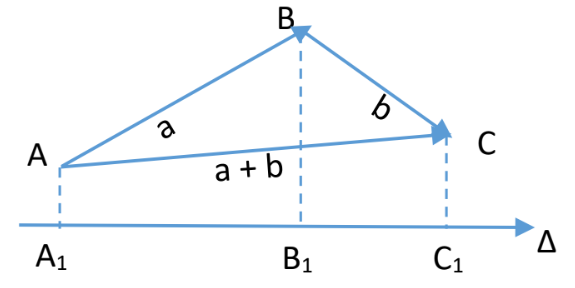
\includegraphics[scale=0.5]{images/triangle2_3.png}
		\end{center}
		Заметим, что
		\begin{enumerate}
			\item $\text{ПР}_\Delta (a+b) = A_1 C_1$,
			\item $\text{ПР}_\Delta a = A_1 B_1$,
			\item $\text{ПР}_\Delta b = B_1 C_1$.
		\end{enumerate}
		По теореме Шаля, $A_1C_1 = A_1 B_1 + B_1 C_1\Rightarrow \text{ПР}_\Delta(a+b) = \text{ПР}_\Delta a + \text{ПР}_\Delta b$.
	\end{Proof}
\end{enumerate}
\newtheorem*{th2_3_1}{Теорема}\begin{th2_3_1}Декартовы координаты вектора равны величинам проекции этого вектора на координатные
	оси.
\end{th2_3_1}\begin{Proof}
	Пусть $a$ --- некоторый вектор пространства с координатами $x, y, z$. Отложим $a$ от начала координат, то есть $а = OM$, а затем построим проекции точки $M$ на оси $Ox, Oy, Oz$. Тогда $\overrightarrow{OM} = \overrightarrow{OM_x} + \overrightarrow{OM_y} + \overrightarrow{OM_z}$. Так как $OM_x \parallel i \parallel Ox$ и, при этом, вектор $i$ ненулевой, он является базисом и $\overrightarrow{OM_x}$ представим в виде: $\overrightarrow{OM_x} = l\cdot i$.\\\\
	Из определения произведения вектора на число, $|\overrightarrow{OM_x}| = |l|\cdot|i|$. Следовательно, $|l| = \dfrac{|\overrightarrow{OM_x}}{|i|} = [|i| = 1] = |\overrightarrow{OM_x}| = |\overline{OM_x}|$, а по знаку $l = \begin{cases}
		|OM_x|, \overline{OM_x} \uparrow\uparrow Ox,\\
		-|OM_x|, \overline{OM_x} \uparrow\downarrow Ox.\\
	\end{cases}\Rightarrow$ по определению проекции, $l = OM_x = \text{ПР}_{Ox}\cdot OM = \text{ПР}_{Ox}\cdot a$.\\\\
	Аналогично $OM_y = \text{ПР}_{Oy}\cdot a, OM_z = \text{ПР}_{Oz}\cdot a\Rightarrow a = \text{ПР}_{Ox}\cdot i + \text{ПР}_{Oy}\cdot j + \text{ПР}_{Oz}\cdot k$. А так как разложение по базису единственно, то $\text{ПР}_{Ox}\cdot a = x, \text{ПР}_{Oy}\cdot a = y, \text{ПР}_{Oz}\cdot a = z$.
\end{Proof}
\newtheorem*{cor2_3_1}{Следствие}\begin{cor2_3_1}Длина вектора $a$ с координатами $(x, y, z)$ равна $\sqrt{x^2 + y^2 + z^2}$.
\end{cor2_3_1}\begin{Proof}
	Из параллелепипеда, построенного на отрезках $OM_x, OM_y, OM_z$, получаем $|a| = |\overline{OM}| = \sqrt{|\overline{OM_x}|^2 + |\overline{OM_y}|^2 + |\overline{OM_z}|^2} = \sqrt{x^2 + y^2 + z^2}$.
\end{Proof}\\\\
Обозначим через $\alpha, \beta$ и $\gamma$ углы между вектор $a$ и векторами $i, j$ и $k$ соответственно.\\\\
$\bullet$ \textit{Числа $cos(\alpha), cos(\beta)$ и $cos(\gamma)$ называются \textbf{направляющими косинусами вектора~ $a$}.}
\newtheorem*{cor2_3_2}{Следствие}\begin{cor2_3_2}$cos^2(\alpha) + cos^2(\beta) + cos^2(\gamma) = 1.$
\end{cor2_3_2}\begin{Proof}
	По теореме, $x = \text{ПР}_{Ox}\cdot a = |a|\cdot cos(a, Ox) = |a|\cdot cos(a, i) = |a|\cdot cos(\alpha)\Rightarrow cos(\alpha) = \dfrac{x}{|a|}$.\\\\
	Аналогично найдем $cos(\beta) = \dfrac{y}{|a|}, cos(\gamma) = \dfrac{z}{|a|}\Rightarrow cos^2(\alpha) + cos^2(\beta) + cos^2(\gamma) = \dfrac{x^2 + y^2 + z^2}{|a|^2} =~ 1$.
\end{Proof}\\\\
$\bullet$ \textit{Единичный вектор, сонаправленный с $a$, называется \textbf{ортом} вектора $a$, и имеет
	координаты $e_a = (cos(\alpha), cos(\beta), cos(\gamma))$}.\\\\
$\bullet$ \textit{Пусть $M$ --- некоторая точка пространства. Вектор $OM$ называется \textbf{радиус-вектором} точки $M$.
	Обозначение: $r_m$.}
\newtheorem*{th2_3_2}{Теорема}\begin{th2_3_2}Радиус-вектор точки $M$ с координатами $(x_m, y_m, z_m)$ имеет такие же координаты $(x_m, y_m, z_m)$.
\end{th2_3_2}\begin{Proof}
	Разложим $r_m$ по базису $i, j, k: r_m = x\cdot i + y\cdot j + z\cdot k$. По первой теореме параграфа, $x_m = OM_x\Rightarrow x = x_m$. Аналогично $y = y_m, z = z_m$. 
\end{Proof}
\newtheorem*{cor2_3_3}{Следствие}\begin{cor2_3_3}Пусть $M_1(x_1, y_1, z_1)$ и $M_2(x_2, y_2, z_2)$ --- две различные точки пространства. Тогда вектор $M_1M_2$ имеет координаты $(x_2 - x_1, y_2 - y_1, z_2 - z_1)$.
\end{cor2_3_3}\begin{Proof}
	$OM_1 + M_1M_2 = OM_2\Rightarrow M_1 M_2 = OM_2 - OM1 = r_{m_2} - r_{m_1}\Rightarrow$ координаты вектора $M_1M_2$ равны $(x_2 - x_1, y_2 - y_1, z_2 - z_1)$.
\end{Proof}







\section{Скалярное произведение векторов.}
$\bullet$ \textit{\textbf{Скалярным произведением} векторов $a$ и $b$ называется число, равное произведению длин этих векторов на косинус угла между ними. Обозначение: $(a, b)$ = $|a|\cdot|b|\cdot cos(a,b)$.}\\\\
\textbf{\textit{Свойства скалярного произведения:}}\begin{enumerate}
	\item \textit{$a$ $\cdot$ $b$ = $b$ $\cdot$ $a$.}
	\begin{Proof} Доказательство следует из определения скалярного произведения.\end{Proof}
	\item $\forall a, b \ne 0\quad a\cdot b$ = $|a| \cdot\text{ПР}_a \cdot b$ = $|b| \cdot\text{ПР}_b \cdot a$.
	\begin{Proof} $a\cdot b$ = $|a| \cdot |b| \cdot cos(a,b)$ = $[$по свойствам величины проекции = ПР$_a \cdot b$ = $|b| \cdot cos(a, b)]$ = $|a| \cdot\text{ПР}_a \cdot b$ \end{Proof}
	\item \textit{$(\lambda\cdot a)\cdot b = \lambda\cdot( a\cdot b) = a\cdot(\lambda\cdot b)$.}
	\begin{Proof} $(\lambda\cdot a )\cdot b = |b| \cdot\text{ПР}_b \cdot(\lambda\cdot a) =|b|\cdot\lambda\cdot\text{ПР}_b\cdot a = \lambda\cdot(a\cdot b)$.\end{Proof}
	\item $(a+b)\cdot c = a\cdot c + b\cdot c, \ \ a\cdot (b+c) = a\cdot b + a\cdot c.$
	\begin{Proof} $(a+b)\cdot c = |c|\cdot\text{ПР}_c\cdot(a+b) = |c|\cdot(\text{ПР}_c\cdot a+\text{ПР}_c\cdot b) = |c|\cdot\text{ПР}_c\cdot a + |c|\cdot\text{ПР}_c\cdot b = a\cdot c + b\cdot c$. \end{Proof}
	\item\textit{$a\cdot a$ $\geqslant$ $0$, причем $a\cdot a = 0$ $\Longleftrightarrow$ $a$ --- нулевой вектор.}
	\begin{Proof} $a\cdot a = |a|\cdot|a|\cdot\underbrace{cos(a,a)}_{=1} = |a|^2 \geqslant 0$, причем $|a|^2 = 0 \Longleftrightarrow |a| = 0$, то есть вектор $a$ --- нулевой. \end{Proof}
	\item\textbf{Критерий перпендикулярности векторов}: \textit{два ненулевых вектора $a$ и $b$ перпендикулярны $\Longleftrightarrow$ их скалярное произведение равно $0$.}
	\begin{Proof} $\Rightarrow$) Пусть $a$ $\perp$ $b$ $\Rightarrow$ $\angle$ $(a, b)$ = $\dfrac{\pi}{2}$ $\Rightarrow$ $a$ $\cdot$ $b$ = $|a|$ $\cdot$ $|b|$ $\cdot$ $cos\dfrac{\pi}{2}$ = $0$.\\\\
		$\Leftarrow$) Пусть $a$ $\cdot$ $b$ = $0$ $\Rightarrow$ $|a|$ $\cdot$ $|b|$ $\cdot$ $cos(a,b)$ = $0$ $\Rightarrow$ $cos(a, b) = 0$ $\Rightarrow$ $\angle$ $(a,b) =$ $\dfrac{\pi}{2}$. \end{Proof}
\end{enumerate}
\newtheorem*{th2_4}{Теорема}\begin{th2_4} Скалярное произведение векторов $a$ и $b$, имеющих декартовы координаты $a(x_1, y_1, z_1)$, $b(x_2, y_2, z_2)$, равно $a\cdot b = x_1\cdot x_2 + y_1\cdot y_2 + z_1 \cdot z_2$.
\end{th2_4}
\begin{Proof}
	По определению декартовых координат, $a$ = $x_1$ $\cdot$ $i$ $+$ $y_1$ $\cdot$ $j$ $+$ $z_1$ $\cdot$ $k$, $b$ $=$ $x_2$ $\cdot$ $i$ $+$ $y_2$ $\cdot$ $j$ $+$ $z_2$ $\cdot$ $k$,
	где $i$, $j$, $k$ --- ортонормированный базис.
	\\ $a$ $\cdot$ $b$ $=$ ($x_1$ $\cdot$ $i$ $+$ $y_1$ $\cdot$ $j$ $+$ $z_1$ $\cdot$ $k$) $\cdot$ ($x_2$ $\cdot$ $i$ $+$ $y_2$ $\cdot$ $j$ $+$ $z_2$ $\cdot$ $k$) $=$ $x_1$ $\cdot$ $x_2$ $\cdot$ $i$ $\cdot$ $i$ $+$ $x_1$ $\cdot$ $y_2$ $\cdot$ $i$ $\cdot$ $j$ $+$ $x_1$ $\cdot$ $z_2$ $\cdot$ $i$ $\cdot$ $k$ $+$ $\dots$ $=$ $[$ $i\cdot j = j\cdot k = i\cdot k = 0$, так как они друг с другом
	перпендикулярны, а $i\cdot i = j\cdot j = k\cdot k = 1$, так как орты, а $cos = 1$ $]$ $=$
	$x_1$ $\cdot$ $x_2$ $+$ $y_1$ $\cdot$ $y_2$ $+$ $z_1$ $\cdot$ $z_2$.
\end{Proof}








\section{Векторное произведение векторов.}
Рассмотрим упорядоченную тройку некомпланарных векторов $e_1, e_2, e_3$, отложим их от некоторой точки $O$ и пусть $e_1$ = $\overrightarrow{O E_1}$, $e_2$ = $\overrightarrow{O E_2}$, $e_3$ = $\overrightarrow{O E_3}$.\\\\
$\bullet$\textit{ Если при наблюдении с конца направленного отрезка $O E_3$ кратчайший поворот от $\overrightarrow{O E_1}$ к $\overrightarrow{O E_2}$ осуществляется против часовой стрелки, то тройка векторов $e_1, e_2, e_3$ называется \textit{\textbf{правой}}, в противном случае \textit{\textbf{левой}}. Данное свойство также называется \textbf{ориентацией} векторов.}
\begin{center}
	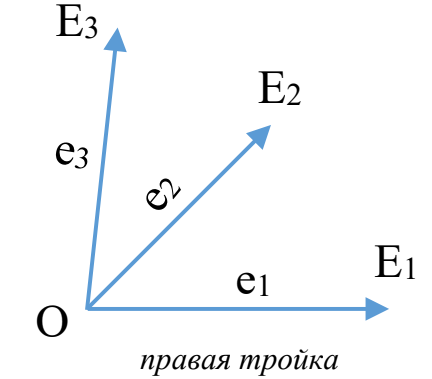
\includegraphics[scale=0.4]{images/r_t_3_5.png}\qquad\qquad\qquad
	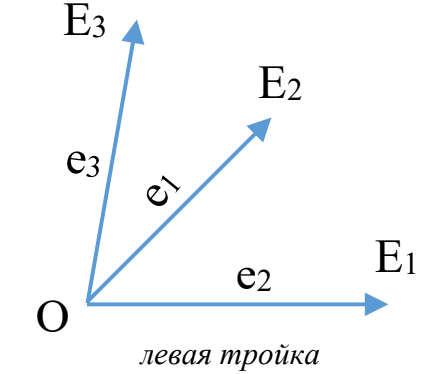
\includegraphics[scale=0.4]{images/l_t_3_5.png} 
\end{center}
Из векторов $a, b,c$ можно составить 6 упорядоченных троек:  \begin{center}
	$a, b, c$ $\hspace{0.5 cm}$ $b, c, a$ $\hspace{0.5 cm}$ $c, a, b$ --- правая тройка; \\
	$a, c, b$ $\hspace{0.5 cm}$ $b, a, c$ $\hspace{0.5 cm}$ $c, b, a$ --- левая тройка.
\end{center}
Из определения ориентации тройки векторов следует, что первые три тройки имеют одну ориентацию, а вторые три противоположную им ориентацию.\\\\
$\bullet$ \textit{\textbf{Векторным произведением} вектора $a$ на вектор $b$ называется вектор, обозначаемый $a$ $\times$ $b$ или $[a, b]$, который удовлетворяет следующим условиям:} 
\begin{enumerate}
	\item |$[a, b]$| = $|a|$ $\cdot$ $|b|$ $\cdot$ $sin (a, b)$;
	\item $[a, b]$ $\perp$ $a$,  $[a, b]$ $\perp$ $b$;
	\item \textit{упорядоченная тройка $a, b, [a, b]$ является правой}.
\end{enumerate}
\textit{\textbf{Свойства векторного произведения векторов:}}
\begin{enumerate}
	\item \textit{Длина векторного произведения векторов $a$ и $b$ равна площади параллелограмма, построенного на векторах $a$ и $b$, отложенных от одной точки}.\begin{Proof}
		Следует из первого пункта определения.
	\end{Proof}
	\item \textit{Два ненулевых вектора $a$ и $b$ коллинеарны $\Longleftrightarrow$ их векторное произведение равно нулевому вектору}.
	\begin{Proof}
		$\Rightarrow$) Пусть векторы $a$ и $b$ коллинеарны, тогда угол между ними в радианах либо 0, либо $\pi$ $\Rightarrow$ $sin (a, b)$ = 0 $\Rightarrow$ $|[a, b]|$ = $|a|$ $\cdot$ $|b|$ $\cdot$ 0 = 0, получили нулевой вектор. \\
		$\Leftarrow$) Пусть векторное произведение $[a, b]$ = $\overrightarrow{0}$ $\Rightarrow$ $|[a, b]|$ = 0 $\Rightarrow$ $|a| \cdot|b|\cdot sin(a, b)$ = 0 ($|a|, |b|$ $\not=$ 0) $\Rightarrow$ $sin (a, b)$ = 0 $\Rightarrow$ $\angle$$(a, b)$ = 0 или $\angle$$(a, b)$ = $\pi$ $\Rightarrow$ $a, b$ коллениарны.
	\end{Proof}
	\item $[a, b] = - [b, a]$.
	\begin{Proof}
		Если векторы $a$ и $b$ коллениарны, то утверждение очевидно. Так как $[a, b]=\overrightarrow{0}$ по второму свойству и, следовательно, $[b, a]=\overrightarrow{0}$.\\\\
		Пусть векторы $a$ и $b$ неколлениарны, тогда векторы $[a, b]$ и $[b, a]$ коллениарны, так как каждый из них одновременно перпендикулярен векторам $a$ и $b$, и, при этом, длины их равны. \begin{center}
			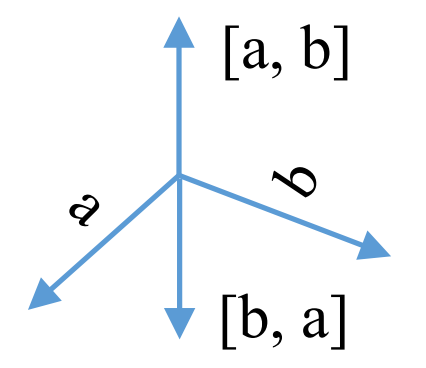
\includegraphics[scale=0.3]{images/vecs_3_5.png}
		\end{center}
		Следовательно, возможны два варианта:
		\begin{enumerate}
			\item $[a, b] = [b, a]$;
			\item $[a, b] = -[b, a]$.
		\end{enumerate}
		Пусть $[a, b] = [b, a]$. По определению векторного произведения, тройка векторов $(a, b, [a, b])$ правая $\Rightarrow$ $(a, b, [b, a])$ тоже правая, но, по определению векторного произведения, тройка векторов $(b, a, [b, a])$ также правая. Тогда, глядя со стороны направления вектора $b$ на $a$, кратчайший поворот против часовой стрелки осуществляется, с одной стороны, от $a$ к $b$, а с другой --- от $b$ к $a$, что является противоречием $\Rightarrow$ $[a, b] = -[b, a]$.
	\end{Proof}
	\item $[\lambda a, b] = \lambda[a, b],\ [a, \lambda b] = \lambda[a, b]\quad \lambda \in \mathbb{R}.$
	\begin{Proof}
		Если векторы $a$ и $b$ коллениарны или $\lambda$ = 0, то утверждение очевидно.\\\\
		Пусть $\lambda$ $\not=$ 0 и векторы $a$ и $b$ неколлениарны. Тогда покажем равенство длин для обоих случаев:\\
		$|\lambda[a, b]| = |\lambda|\cdot|[a, b]| = |\lambda|\cdot|a|\cdot|b|\cdot sin(a, b)$. \\
		$|[\lambda a, b]| = |\lambda a|\cdot|b|\cdot sin(\lambda a, b) = \begin{cases} |\lambda|\cdot|a|\cdot|b|\cdot sin (a, b),\ \lambda > 0; \\  |\lambda|\cdot|a|\cdot|b|\cdot sin (\pi - \angle (a, b)),\ \lambda < 0.\end{cases} = |\lambda|\cdot|a|\cdot|b|\cdot sin (a, b)$. \\\\
		Покажем направления: \\
		$[\lambda a, b]$ и $\lambda[a, b]$ перпендикулярны и $a$, и $b$ $\Rightarrow$ $[\lambda a, b]$ $\parallel$ $\lambda[a, b]$. При $\lambda$ > 0 векторное произведение $[a, b]$ сонаправлено с обоими векторами $a, b$. \\
		При $\lambda$ < 0 векторное произведение $[a, b]$ имеет противоположное направление с векторами $a, b$ $\Rightarrow$ \\ $[\lambda a, b]$ $\uparrow\downarrow$ $\lambda[a, b]$ $\Rightarrow$ $[a, \lambda b] = -[\lambda b, a] = -\lambda [b, a] = \lambda [a, b]$.
	\end{Proof}
	\item \begin{enumerate}
		\item[$a$)] $[a + b, c] = [a, c] + [b, c]$;
		\item[$b$)] $[a, b + c] = [a, b] + [a, c]$.
	\end{enumerate}
	\begin{Proof} \begin{enumerate}
			\item Если один из векторов $a, b, c$ нулевой, то утверждение очевидно.\\\\
			Пусть векторы $a, b, c$ ненулевые. Обозначим через $e_c$ орт вектора $c$, тогда $e_c$ = $\dfrac{1}{|c|}$ $\cdot$ $c$ $\Rightarrow$ $|e_c|$ = 1. \\
			Построим векторное произведение вектора $a$ на $e_c$ следующим образом:
			\begin{enumerate}
				\item [1)]отложим векторы $a$ и $e_c$ от некоторой точки $O$. Тогда $a$ = $\overrightarrow{OA}$, $e_c$ = $\overrightarrow{OC}$; 
				\item [2)] проведем через точку $O$ плоскость перпендикулярно отрезку $OC$;
				\item [3)] построим отрезок $O A_1$ --- проекцию отрезка $OA$ на плоскость П, а затем повернем этот отрезок в плоскости П вокруг точки $O$ по часовой стрелке на угол $\dfrac{\pi}{2}$ и получим отрезок $O A_2$.
			\end{enumerate}\begin{center}
				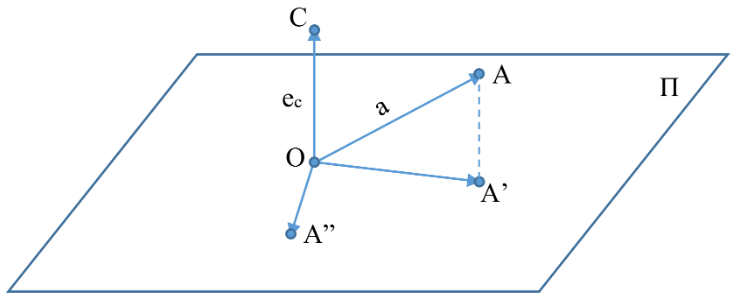
\includegraphics[scale=0.4]{images/pl_3_5.png}
			\end{center}
			Докажем, что $\overrightarrow{O A_2}$ = $[\overrightarrow{OA}, \overrightarrow{OC}]$ = $[a, e_c]$.
			\begin{enumerate}
				\item [1)] Длина: $|\overrightarrow{O A_2}| = |\overline{O A_2}| = |\overline{O A_1}| = |\overline{OA}|\cdot cos \angle AO A_1 = |\overline{OA}| \cdot cos (\pm (\dfrac{\pi}{2} - \angle(a, e_c)) = |a|\cdot|e_c|\cdot sin (a, e_c) = |[a, e_c]|$.\\
				\item [2)] Направление: $\overline{O A_2}$ $\perp$ $\overline{OC}$, так как $\overline{OA_2}$ лежит в плоскости, перпендикулярной отрезку $OC$, $\overline{O A_2}$ $\perp$ $\overline{OA}$ $\Rightarrow$ $\overline{O A_2}$ $\perp$ $e_c$, $\overline{O A_2}$ $\perp$ $a$ по теореме о трех перпендикулярах.\\
				\item [3)] Тройка векторов $\overrightarrow{OA}$, $\overrightarrow{OC}$, $\overrightarrow{O A_2}$ правая по построению.
			\end{enumerate}
			Таким образом мы показали, что $\overrightarrow{O A_2}$ = $[a, e_c]$. \\
			Отложим вектор $b$ от точки $A$. Пусть $b$ = $\overrightarrow{AB}$. Построим треугольник $O A_1 B_1$ --- проекцию треугольника $OAB$ на плоскость П, а затем повернем этот треугольник по часовой стрелке вокруг точки $O$ на угол $\dfrac{\pi}{2}$ и получим треугольник $O A_2 B_2$.
			\begin{center}
				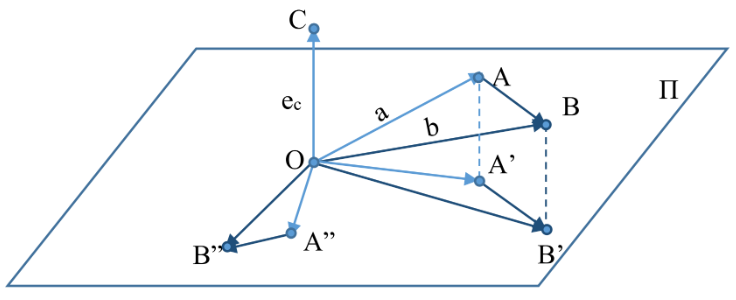
\includegraphics[scale=0.4]{images/pl2_3_5.png}
			\end{center}
			По определению суммы векторов, $\overrightarrow{O B_2} = \overrightarrow{O A_2} + \overrightarrow{A_2 B_2}$. По доказанному выше,
			$\overrightarrow{O B_2}$ = $[\overrightarrow{OB}, \overrightarrow{OC}] = [a + b, e_c]$, 
			$\overrightarrow{A_2 B_2} = [\overrightarrow{AB}, \overrightarrow{OC}] = [b, e_c]$ \\
			Следовательно, из полученного выше имеем $[a + b, e_c] = [a, e_c] + [b, e_c]$. \\
			Домножим полученное равенство на длину вектора $c$ и используем четвертое свойство. Получим $[a + b, c] = [a, c] + [b, c]$.
			\item $[a, b + c]$ = -$[b + c, a]$ = -$([b, a] + [c, a])$ = $[a, b] + [a, c]$.
		\end{enumerate}
	\end{Proof}
\end{enumerate}
$\bullet$ \textit{Квадратная таблица чисел вида} $\begin{pmatrix} \alpha_1 & \alpha_2 \\ \beta_1 & \beta_2 \end{pmatrix}$ \textit{называется \textbf{матрицей второго порядка}}. \\
$\bullet$ \textit{\textbf{Определителем} матрицы второго порядка называется число вида} $\begin{vmatrix} \alpha_1 & \alpha_2 \\ \beta_1 & \beta_2 \end{vmatrix} = \\ = \alpha_1\beta_2 - \alpha_2\beta_1$. \\
\newtheorem*{t3_5_1}{Теорема}\begin{t3_5_1} Пусть векторы $a$ и $b$ в правой ДПСК имеют координаты $a (X_1, Y_1, Z_1)$ и $b (X_2, Y_2, Z_2)$, тогда вектор $[a, b]$ имеет координаты\begin{center}
		$[a, b]$ =  $\Bigg( \begin{vmatrix} Y_1 & Z_1 \\ Y_2 & Z_2 \end{vmatrix}, - \begin{vmatrix} X_1 & Z_1 \\ X_2 & Z_2 \end{vmatrix}, \begin{vmatrix} X_1 & Y_1 \\ X_2 & Y_2 \end{vmatrix} \Bigg)$.
	\end{center}
\end{t3_5_1}
\begin{Proof}
	Из определения декартовых координат вектора следует, что $a$ = $X_1 \cdot i + Y_1 \cdot j + Z_1 \cdot k$, \\ $b$ = $X_2 \cdot i + Y_2 \cdot j + Z_2 \cdot k$. Тогда \\ $[a, b]$ = $[X_1 \cdot i + Y_1 \cdot j + Z_1 \cdot k, \ X_2 \cdot i + Y_2 \cdot j + Z_2 \cdot k]$ = $X_1 \cdot X_2 \cdot [i, i] + X_1 \cdot Y_2 \cdot [i, j] + \\ + X_1 \cdot Z_2 \cdot [i, k] + Y_1 \cdot X_2 \cdot [i, j] + Y_1 \cdot Z_2 \cdot [j, k] + Z_1 \cdot X_2 \cdot [k, i] + Z_1 \cdot Y_2 \cdot [k, j] + Z_1 \cdot Z_2 \cdot [k, k] + Y_1 \cdot Y_2 \cdot [j, j]$. \\\\
	$[i,i]$ = $\overrightarrow{0}$, $[j,j]$ = $\overrightarrow{0}$, $[k,k]$ = $\overrightarrow{0}$, так как векторы параллельны сами себе, следовательно, применимо второе свойство. $[i,j]$ = $k$, $[i,k]$ = $-j$, $[j,i]$ = $-k$,  $[j,k]$ = $i$, $[k,i]$ = $j$, $[k,j] = -i$. \\\\
	Подставим и получим $X_1 \cdot Y_2 \cdot k + X_1 \cdot Z_2 \cdot (-j) + Y_1 \cdot X_2 \cdot (-k) + Y_1 \cdot Z_2 \cdot i + Z_1 \cdot X_2 \cdot j + Z_1 \cdot Y_2 \cdot (-i)$ = $(Y_1 \cdot Z_2 - Z_1 \cdot Y_2) \cdot i$ - $(X_1 \cdot Z_2 - Z_1 \cdot X_2) \cdot j$ + $(X_1 \cdot Y_2 - Y_1 \cdot X_2) \cdot k$ = \\ = $\begin{vmatrix} Y_1 & Z_1 \\ Y_2 & Z_2 \end{vmatrix} \cdot i - \begin{vmatrix} X_1 & Z_1 \\ X_2 & Z_2 \end{vmatrix} \cdot j + \begin{vmatrix} X_1 & Y_1 \\ X_2 & Y_2 \end{vmatrix} \cdot k$.
\end{Proof}




\section{Смешанное произведение векторов.}
$\bullet$ \textit{\textbf{Смешанным произведением трех векторов a, b, c} называется число $abc = [a,b]\cdot c$.}
\newtheorem*{th2_6_1}{Теорема}\begin{th2_6_1}
	Пусть $V$ --- объём параллелепипеда, построенного на отложенных от одной точки трех некомпланарных векторах $a$, $b$, $c$. Тогда $abc = \begin{cases} V\text{, где a,b,c --- правая тройка}; \\  
		-V\text{, где a,b,c  --- левая тройка}. \end{cases}$ \end{th2_6_1}
\begin{Proof}
	Пусть векторы $a,b$ и $c$ отложены от точки $O$. Тогда $a$ = $\overrightarrow{OA}$, $b$ = $\overrightarrow{OB}$ и $c$ = $\overrightarrow{OC}$. Так как векторы $a, b, c$ некомпланарны, то векторы $a$ и $b$ неколлениарны.\\
	\begin{center}
		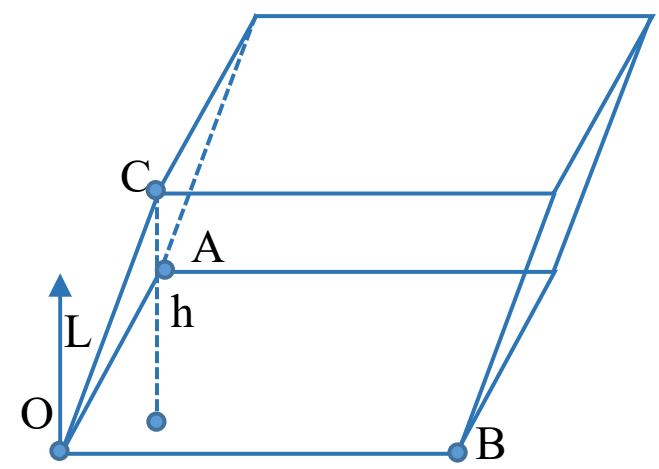
\includegraphics[scale=0.2]{images/par_2_6.png}
	\end{center}
	Обозначим через $S$ площадь параллелограмма, построенного на отрезках $OA$ и $OB$. Тогда $S$ = $|\overrightarrow{OA}|\cdot|\overrightarrow{OB}|\cdot sin \angle (BOA) = |a| \cdot |b| \cdot sin(a, b) = |[a, b]|$. \\\\
	Обозначим через $e$ орт $[a, b]$. Тогда тройка векторов $a, b, c$ --- правая и при этом \\ $[a, b] = |[a, b]|\cdot e = S \cdot e$ $\Rightarrow$ $abc = [a, b]\cdot c = (S \cdot e) \cdot c = S \cdot (e \cdot c) = S\cdot|e|\cdot\text{ПР}_e c = S\cdot\text{ПР}_e c$. \\\\
	Пусть $h$ --- высота рассматриваемого параллелепипеда, опущенная из вершины $C$ на плоскость $AOB$, тогда $|\text{ПР}_{e}c| = h$, \\ но при этом $\begin{cases} \text{ПР}_ec > 0\text{, если $a, b, c$ --- правая тройка векторов};\\ \text{ПР}_{e}c < 0\text{, если $a, b, c$ --- левая тройка векторов}. \end{cases} \Rightarrow \\ abc = \begin{cases} abc = S\cdot h\text{, если $a, b, c$ --- правая тройка}; \\  abc = -S\cdot h\text{, если $a, b, c$  --- левая тройка}. \end{cases} \Rightarrow V = |abc|$ и условие теоремы выполняется.
\end{Proof}\\\\
\textit{\textbf{Свойства смешанного произведения:}}
\begin{enumerate}
	\item \textit{Векторы $a, b, c$ компланарны $\Longleftrightarrow$ их смешанное произведение $abc = 0$}.
	\begin{Proof}
		$\Rightarrow$) Пусть векторы $a, b, c$ компланарны.
		\begin{enumerate}
			\item [1)] $a \parallel b \Rightarrow [a, b] = 0 \Rightarrow abc = [a, b]\cdot c = 0$; 
			\item [2)] $a \nparallel b \Rightarrow [a, b] \perp a, [a, b] \perp b \Rightarrow [a, b] \perp c \Rightarrow abc = [a, b]\cdot c = 0$. 
		\end{enumerate}
		$\Leftarrow$) Пусть $abc$ = 0, и предположим, что векторы $a, b, c$ некомпланарны. Тогда, отложив их от одной точки, можно построить параллелепипед с $V$ = $|abc|$ $\not=$ 0, что противоречит тому, что $abc = 0$. Значит $a, b, c$ компланарны.
	\end{Proof}
	\item $abc = bca = cab = -acb = -bac = -cba$.
	\begin{Proof}
		Если векторы $a, b, c$ компланарны, то все произведения равны 0. \\
		Если векторы $a, b, c$ некомпланарны, то модули рассматриваемых смешанных произведений будут равны, а знак зависит от ориентации соответствующих троек. \\
		Первые три смешанных произведений имеют одну ориентацию, а последние три противоположную ориентацию.
	\end{Proof}
	\item $(\alpha a) bc = a (\alpha b) c = ab (\alpha c) = \alpha (abc)$.
	\begin{Proof}
		$ab(\alpha c) = [a, b] (\alpha c) = \alpha ([a, b] c) = \alpha (abc)$.
	\end{Proof}
	\item $(a + b) \cdot c \cdot d = acd + bcd;$ \\
	$a \cdot (b + c) \cdot d = abd + acd;$ \\
	$a \cdot b \cdot (c + d) = abc + abd.$
	\begin{Proof}
		$(a + b) \cdot c \cdot d = [a + b, c] \cdot d = ([a, c] + [b, c]) \cdot d = [a, c] \cdot d + [b, c] \cdot d = acd + bcd$.
	\end{Proof}
\end{enumerate}
$\bullet$ \textit{Квадратная таблица чисел вида} $\begin{pmatrix} \alpha_1 & \alpha_2 & \alpha_3 \\ 
	\beta_1 & \beta_2 & \beta_3 \\ \gamma_1 & \gamma_2 & \gamma_3 \end{pmatrix}$ \textit{называется \textbf{матрицей третьего порядка}}.\\
$\bullet$ \textit{\textbf{Определителем} матрицы третьего порядка является число вида} $\begin{vmatrix} \alpha_1 & \alpha_2 & \alpha_3 \\ 
	\beta_1 & \beta_2 & \beta_3 \\ \gamma_1 & \gamma_2 & \gamma_3 \end{vmatrix} = \\ = \alpha_1 \begin{vmatrix} \beta_1 & \beta_3 \\ \gamma_2 & \gamma_3 \end{vmatrix} - \alpha_2 \begin{vmatrix} \beta_1 & \beta_3 \\ \gamma_1 & \gamma_3 \end{vmatrix} + \alpha_3 \begin{vmatrix} \beta_1 & \beta_2 \\ \gamma_1 & \gamma_2 \end{vmatrix}$. \\\\
\newtheorem*{t3_6_2}{Теорема}\begin{t3_6_2}
	Пусть векторы $a, b, c$ в правой ДПСК имеют координаты $a(x_1, y_1, z_1)$, $b(x_2, y_2, z_2)$, $c(x_3, y_3, z_3)$, тогда $abc = \begin{vmatrix} x_1 & y_1 & z_1 \\ x_2 & y_2 & z_2 \\ x_3 & y_3 & z_3 \end{vmatrix}$. \end{t3_6_2}
\begin{Proof}
	$abc = bca = [b, c] \cdot a = \Bigg( \begin{vmatrix} Y_2 & Z_2 \\ Y_3 & Z_3 \end{vmatrix}, - \begin{vmatrix} X_2 & Z_2 \\ X_3 & Z_3 \end{vmatrix}, \begin{vmatrix} X_2 & Y_2 \\ X_3 & Y_3 \end{vmatrix} \Bigg) \cdot (x_1, y_1, z_1) = \\ = x_1 \begin{vmatrix} Y_2 & Z_2 \\ Y_3 & Z_3 \end{vmatrix} - y_1 \begin{vmatrix} X_2 & Z_2 \\ X_3 & Z_3 \end{vmatrix} + z_1 \begin{vmatrix} X_2 & Y_2 \\ X_3 & Y_3 \end{vmatrix} = \begin{vmatrix} X_1 & Y_1 & Z_1 \\ X_2 & Y_2 & Z_2 \\ X_3 & Y_3 & Z_3 \end{vmatrix}$.
\end{Proof}





\section{Преобразование декартовых прямоугольных координат на плоскости и в пространстве.}
Пусть на плоскости заданы две ДПСК: $Oxy$, $O'x'y'$ и пусть некоторая точка $M$ плоскости в первой ДПСК имеет координаты $(x, y)$, а во второй $(x', y')$. Выразим координаты $(x, y)$ через $(x', y')$. \\\\Пусть $i, j, i', j'$ --- направляющие орты осей координат $Ox, Oy, O'x', O'y'$ соответственно. Так как точка $M$ в ДПСК $Oxy$ имеет координаты $(x, y)$, то вектор $\overrightarrow{OM}$ представим в виде $\overrightarrow{OM}$ = $x \cdot i$ + $y \cdot j$.
Аналогично $\overrightarrow{O' M}$ = $x' \cdot i'$ + $y' \cdot j'$. \\\\
Пусть точка $O'$ в исходной ДПСК имеет координаты $(a, b)$, тогда $\overrightarrow{O O'}$ = $a \cdot i$ + $b \cdot j$. \\\\
Так как любой вектор можно разложить по базису на плоскости, то векторы $i'$, $j'$ можно разложить по базисам $i$, $j$ на плоскости, то есть представить в виде $i'$ = $\alpha_1 \cdot i + \alpha_2 \cdot j$, \\ $j'$ = $\beta_1 \cdot i + \beta_2 \cdot j$. \\\\Определим коэффициенты этих разложений. Для этого умножим каждое равенство на векторы $i, j$: \\
$i'\cdot i$ = $\alpha_1 \cdot i \cdot i$ + $\alpha_2 \cdot j \cdot i$ = $\alpha_1$ $\Rightarrow$ $\alpha_1$ = $i' \cdot i$ = $|i'| \cdot |i| \cdot cos(i, i')$ = $cos(i, i')$ \\
$i' \cdot j$ = $\alpha_1 \cdot i \cdot j$ + $\alpha_2 \cdot j \cdot j$ $\Rightarrow$ $\alpha_2$ = $i' \cdot j$ = $|i'| \cdot |j| \cdot cos(j, i')$ \\
$j' \cdot i$ = $\beta_1 \cdot i \cdot i$ + $\beta_2 \cdot j \cdot i$ = $\beta_1$ $\Rightarrow$ $\beta_1$ = $j' \cdot i$ =  $cos(i, j')$ \\
$j' \cdot j$ = $\beta_1 \cdot i \cdot j$ + $\beta_2 \cdot j \cdot j$ = $\beta_2$ $\Rightarrow$ $\beta_2$ = $j' \cdot j$ =  $cos(j, j')$ \\\\
Из определения суммы векторов следует, что
$\overrightarrow{OM}$ = $\overrightarrow{O O'}$ + $\overrightarrow{O' M}$. Тогда из разложения по базису этих векторов получим \\
$x \cdot i$ + $y \cdot j$ = $a\cdot i + b\cdot j + x' \cdot (\alpha_1 \cdot i + \alpha_2 \cdot j) + y'\cdot (\beta_1 \cdot i + \beta_2 \cdot j)$ ; \\
$x \cdot i$ + $y \cdot j$ = ($a + x' \cdot \alpha_1 + y' \cdot \beta_1$) $\cdot$ $i$ + ($b + x' \cdot \alpha_2 + y' \cdot \beta_2$) $\cdot$ $j$. \\\\
Так как разложение любого вектора по базису единственно, то  $\begin{cases}
	x = a + x' \cdot \alpha_1 + y' \cdot \beta_1, \\
	y = b + x' \cdot \alpha_2 + y' \cdot \beta_2.
\end{cases}\Rightarrow$ $$\begin{cases}
	x = a + x' \cdot cos(i, i') + y' \cdot cos(i, j'),\\
	y = b + x' \cdot cos(j, i') + y' \cdot cos(j, j').
\end{cases}\eqno (2.7.1)$$\\\\
$\bullet$ \textit{Полученная формула $(2.7.1)$ называется \textbf{формулой преобразования декартовых координат точки}.}\\\\
Рассмотрим некоторые частные случаи.
\begin{enumerate}
	\item \textbf{Преобразование симметрии относительно прямой $(y = x)$.} \\
	Пусть точки $O(x,y)$ и $O'(x',y')$ --- начала двух ДПСК разной ориентации. И пусть они совпадают $(O = O')$. \begin{center}
		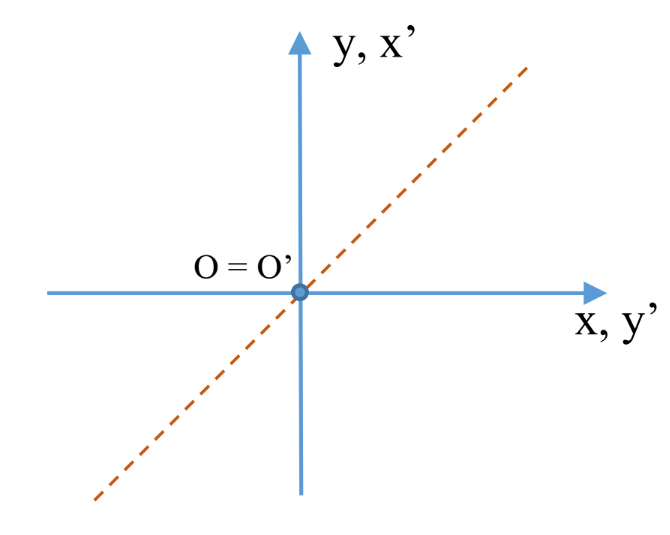
\includegraphics[scale=0.3]{images/dpsk1_2_7.png}
	\end{center}
	Тогда получаем
	$\angle (i, i')$ = $\angle (i, j)$ = $\dfrac{\pi}{2}$, $\angle (j, j')$ = $\angle (j, i)$ = $\dfrac{\pi}{2}$, $\angle (i, j')$ = $\angle (j, i')$ = 0. Отсюда имеем $$\begin{cases} x = y', \\ y = x'. \end{cases}\eqno (2.7.2)$$\\\\
	$\bullet$ \textit{Полученная формула $(2.7.2)$ называется \textbf{формулой преобразования симметрии относительно прямой} $y = x$.}\\
	\item \textbf{Параллельный перенос координатных осей.}\\
	Пусть начало новой ДПСК располагается в точке $O' (a, b)$ исходной ДПСК.\begin{center}
		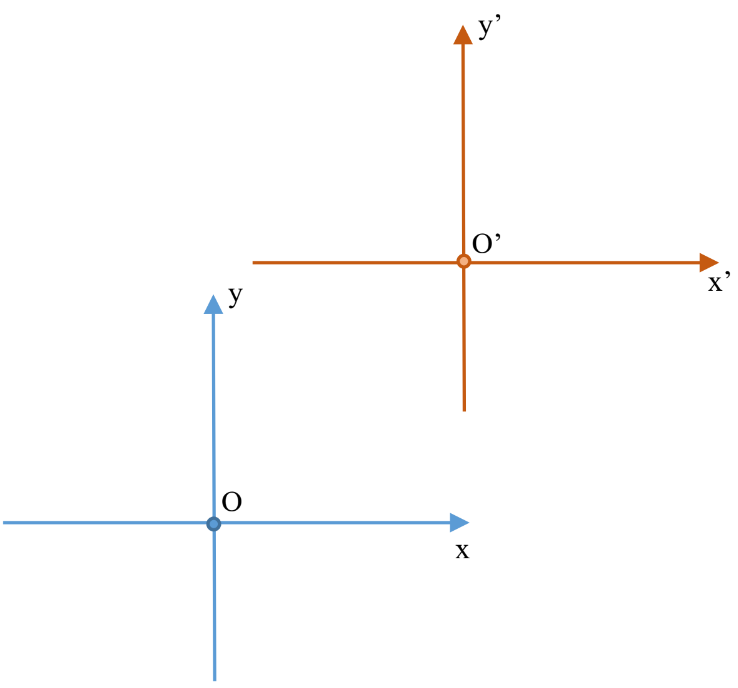
\includegraphics[scale=0.3]{images/dpsk2_2_7.png}
	\end{center}
	При параллельном переносе координатных осей их орты совпадают, то есть $i=i'$, $j=j'$. Тогда \\ $$\begin{cases}
		x = a + x' \cdot cos 0 + y'cos \dfrac{\pi}{2}, \\
		y = b + x' \cdot cos \dfrac{\pi}{2} + y' \cdot sin \dfrac{\pi}{2}.
	\end{cases} \Rightarrow 
	\begin{cases}
		x = a + x', \\
		y = b + y'.
	\end{cases}\eqno(2.7.3)$$\\
	$\bullet$ \textit{Полученная формула $(2.7.3)$ называется \textbf{формулой параллельного переноса}.}\\
	\item \textbf{Преобразование поворота.} \\
	Пусть ДПСК $O'x'y'$ получена из правой ДПСК $Oxy$ путем поворота вокрут точки $O$ против часовой стрелки на угол $\varphi$.
	\begin{center}
		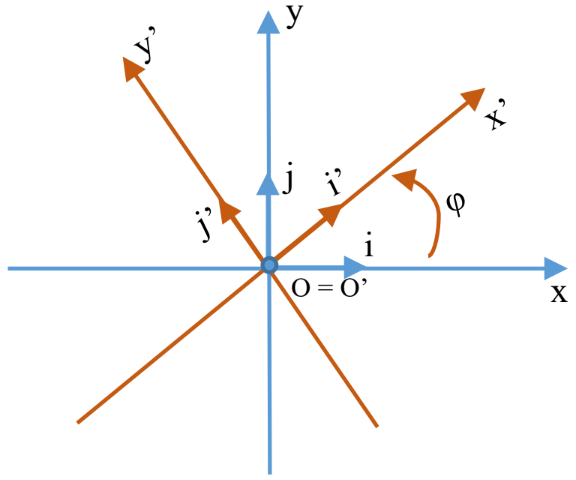
\includegraphics[scale=0.4]{images/dpsk3_2_7.png}
	\end{center}
	И пусть начала координат равны $(O' = O)$. Тогда\\
	$cos (i, i')$ = $cos \varphi$,\\ 
	$cos (i, j')$ = $cos (\varphi + \dfrac{\pi}{2})$,\\ 
	$cos (j, i')$ = $cos (\dfrac{\pi}{2} - \varphi)$,\\ 
	$cos(j, j')$ = $cos \varphi$.\\ 
	Из уравнений выше следует система\\
	$$\begin{cases}
		x = x' cos \varphi - y' sin \varphi, \\
		y = x' sin \varphi + y' cos \varphi.
	\end{cases}\eqno (2.7.4)$$\\
	$\bullet$ \textit{Полученная формула $(2.7.4)$ называется \textbf{формулой преобразования поворота}.}
\end{enumerate}
Пусть точка $M$ в ДПСК $Oxyz$ имеет координаты $(x, y, z)$, а в ДПСК $O'x'y'z'$ ---  $(x', y', z')$, и пусть точка $O$ имеет координаты $O(a, b, c)$ в ДПСК $Oxyz$. Тогда справедлива система
$$\begin{cases}
	x = a + x' cos (i, i') + y' cos (i, j') + z' cos(i, k'), \\
	y = b + x' cos (j, i') + y' cos (j, j') + z' cos(j, k'), \\
	z = c + x' cos (k, i') + y' cos (k, j') + z' cos(k, k').
\end{cases}\eqno(2.7.5)$$\\
$\bullet$ \textit{Полученная формула $(2.7.5)$ называется \textbf{формулой преобразования декартовых координат в пространстве}.}




\chapter{Уравнения прямой на плоскости}

\section{Общее уравнение прямой. Уравнение прямой в отрезках.}
$\bullet$ \textit{\textbf{Нормальным вектором} прямой на плоскости называется ненулевой вектор, перпендикулярный данной прямой.} \\\\
Рассмотрим некоторую прямую $\Delta$. Пусть она проходит через некоторую точку $M_0 (x_0, y_0)$ и она перпендикулярна ненулевому вектору $n(A, B).$
\begin{center}
	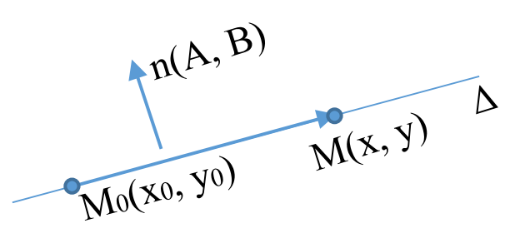
\includegraphics[scale=0.4]{images/line3_1.png}
\end{center}
Так как вектор $n$ ненулевой, то $A^2 + B^2$ $\not=$ 0. Если некоторая точка $M(x, y)$ лежит на прямой $\Delta$, то $\overrightarrow{M_0 M}$ $\perp$ $n$ и наоборот, если точка $M$ не лежит на прямой $\Delta$, то $\overrightarrow{M_0 M}$  $\not \perp$ $n$. \\\\
Таким образом, точка $M$ $\in$ $\Delta$ $\Longleftrightarrow$ $\overrightarrow{M_0 M}$ $\perp$ $n$. \\\\
$\bullet$ \textit{Уравнение $\overrightarrow{M_0 M}$ $\cdot$ $n = 0$ называется \textbf{уравнением в векторной форме прямой на плоскости}, проходящей через точку $M_0$ перпендикулярно вектору $n$.}\\\\
Вектор $\overrightarrow{M_0 M}$ в ДПСК имеет координаты $(x - x_0, y - y_0)$. Тогда $$A(x - x_0) + B(y - y_0) = 0.\eqno (3.1.1)$$
$\bullet$ \textit{Уравнение $(3.1.1)$ называется \textbf{уравнением в координатной форме прямой на плоскости}, проходящей через точку с координатами $(x_0, y_0)$ перпендикулярно вектору $n$ с координатами $(A, B)$.}
\newtheorem*{t4_1_1}{Теорема}\begin{t4_1_1} Любая прямая на плоскости в ДПСК может быть задана уравнением вида
	$$Ax + By + C = 0,\quad A^2 + B^2\ne0.\eqno(3.1.2)$$
	В ДПСК любое уравнение вида $(3.1.2)$ определяет прямую и только.
\end{t4_1_1}
\begin{Proof}
	\begin{enumerate}
		\item Пусть произвольная прямая $\Delta$ проходит через точку $M_0(x_0, y_0)$ перпендикулярно вектору $n(A, B)$. Преобразуем уравнение (3.1.1) следующим образом: $Ax + By$ + $\underbrace{(-Ax_0 - By_0)}_{C}$ = $0$. Тогда уравнение прямой примет вид (3.1.2), причем $A$ и $B$ --- координаты нормального вектора. Следовательно, $A^2 + B^2 \ne 0$.
		\item Так как коэффициенты $A$ и $B$ не обращаются в 0 одновременно, то уравнение (3.1.2) всегда имеет решение. Пусть $(x_0, y_0)$ --- решение уравнения (3.1.2). Тогда $Ax_0 + By_0 + C = 0$.\\
		Вычтем полученное равенство из уравнения (2) и получим $A(x - x_0) + B(y - y_0) = 0$ --- уравнение прямой, проходящей через точку $M_0$. Значит уравнение (3.1.2) является уравнением прямой.
	\end{enumerate}
\end{Proof}\\
$\bullet$ \textit{Уравнение $(3.1.2)$ называется \textbf{общим уравнением прямой на плоскости}. Причем коэффициенты $A$ и $B$ являются координатами нормального вектора $n$.}
\newtheorem*{t4_1_2}{Теорема}\begin{t4_1_2} Если два общих уравнения $\begin{matrix} A_1 x + B_1 y + C_1 = 0, \\ A_2 x + B_2 y + C_2 = 0 \end{matrix}$ определяют одну прямую, то существует действительное число $\lambda$ такое, что $A_1$ = $\lambda\cdot A_2$, $B_1$ = $\lambda\cdot B_2$, $C_1$ = $\lambda\cdot C_2$. \end{t4_1_2}
\begin{Proof}
	Так как оба уравнения описывают одну прямую, то векторы $n_1(A_1, B_1)$ и $n_2(A_2, B_2)$ являются нормальными векторами одной прямой $\Rightarrow$ они коллениарны и $\exists$ $\lambda$ такое, что $A_1 = \lambda\cdot A_2$, а $B_1 = \lambda\cdot B_2$. Пусть прямая проходит через точку $M_0(x_0, y_0)$, тогда подставим и получим следующие уравнения:
	\begin{center}
		$A_1 x_0 + B_2 y_0 + C_1 = 0,$ \\
		$A_2 x_0 + B_2 y_0 + C_2 = 0.$
	\end{center}
	Отнимем от первого уравнения второе домноженное на $\lambda$ и получим \\
	$\underset{= 0}{(A_1 - \lambda A_2)} \cdot x_0 + \underset{= 0}{(B_1 - \lambda B_2)} \cdot y_0 + (C_1 - \lambda\cdot C_2) = 0 \ \Rightarrow C_1 - \lambda C_2 = 0 \Rightarrow C_1 = \lambda C_2$.
\end{Proof} \\\\
Рассмотрим взаимное расположение двух прямых. Пусть $A_1 x + B_1 y + C_1 = 0$ и $A_2 x + B_2 y + C_2 = 0$ --- уравнения этих двух прямых.
\begin{enumerate}
	\item Прямые совпадают, если $\exists$$\lambda$ $\in$ $R$ : $A_1$ = $\lambda$$\cdot$$A_2$, $B_1$ = $\lambda$$\cdot$$B_2$, $C_1$ = $\lambda$$\cdot$$C_2$;
	\item Прямые параллельны, если $\exists$$\lambda$ $\in$ $R$ : $A_1$ = $\lambda$$\cdot$$A_2$, $B_1$ = $\lambda$$\cdot$$B_2$, $C_1$ $\not=$ $\lambda$$\cdot$$C_2$;
	\item Прямые пересекаются, если $\nexists$$\lambda$ $\in$ $R$ : $A_1$ = $\lambda$$\cdot$$A_2$, $B_1$ = $\lambda$$\cdot$$B_2$. Угол пересечения равен углу между нормальными векторами этих прямых, то есть$$cos(\Delta_1, \Delta_2) = \dfrac{|n_1\cdot n_2|}{|n_1| \cdot |n_2|} = \dfrac{|A_1 A_2 + B_1 B_2|}{\sqrt{A_1^2 + B_1^2} \cdot \sqrt{A_2^2 + B_2^2}}.$$
	\begin{center}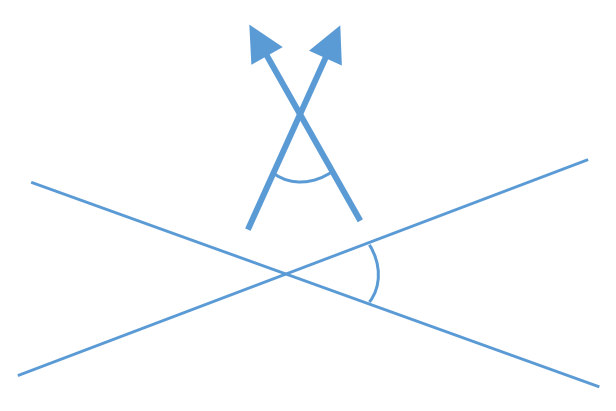
\includegraphics[scale=0.4]{images/corn3_1.png}\end{center}
\end{enumerate}
$\bullet$ \textit{Общее уравнение прямой называется \textbf{полным}, если все его коэффициенты $A, B$ и $C$ $\not=$ 0. В противном случае уравнение называется \textbf{неполным}.} \\\\
Рассмотрим виды неполных уравнений. Пусть $\Delta$ --- прямая.
\begin{enumerate}
	\item $C = 0 \Rightarrow O(0,0) \in \Delta$, прямая проходит через начало координат;
	\item $B = 0 \Rightarrow \Delta \parallel Oy$;
	\item $A = 0 \Rightarrow \Delta \parallel Ox$;
	\item $B = 0, C= 0 \Rightarrow \Delta = Oy$;
	\item $A = 0, C= 0 \Rightarrow \Delta = Ox$.
\end{enumerate}
Рассмотрим полное уравнение $A x + B y + C = 0$. Прямая, описанная этим уравнением, не проходит через начало координат и не параллельна ни одной из координатных осей. Преобразуем уравнение следующим образом:\\
$A x + B y = - C \Rightarrow$ $\dfrac{Ax}{-C}$ + $\dfrac{By}{-C}$  = 1 $\Rightarrow$ $\dfrac{x}{\dfrac{-C}{A}}$ + $\dfrac{y}{\dfrac{-C}{B}}$ = 1 $\Rightarrow\Big[\dfrac{-C}{A}$ = $a$, \ $\dfrac{-C}{B}$ = $b\Big]$ $\Rightarrow$ $$\dfrac{x}{a} + \dfrac{y}{b} = 1.\eqno(3.1.3)$$
$\bullet$ \textit{Уравнение $(3.1.3)$ называется \textbf{уравнением прямой в отрезках}.}\\\\
Так как точки пересечения этой прямой с координатными осями имеют координаты $(a, 0)$ и $(0, b)$, то $a$ и $b$ --- величины направленных отрезков, отсекаемых прямой по координатным осям от начала координат.
\begin{center}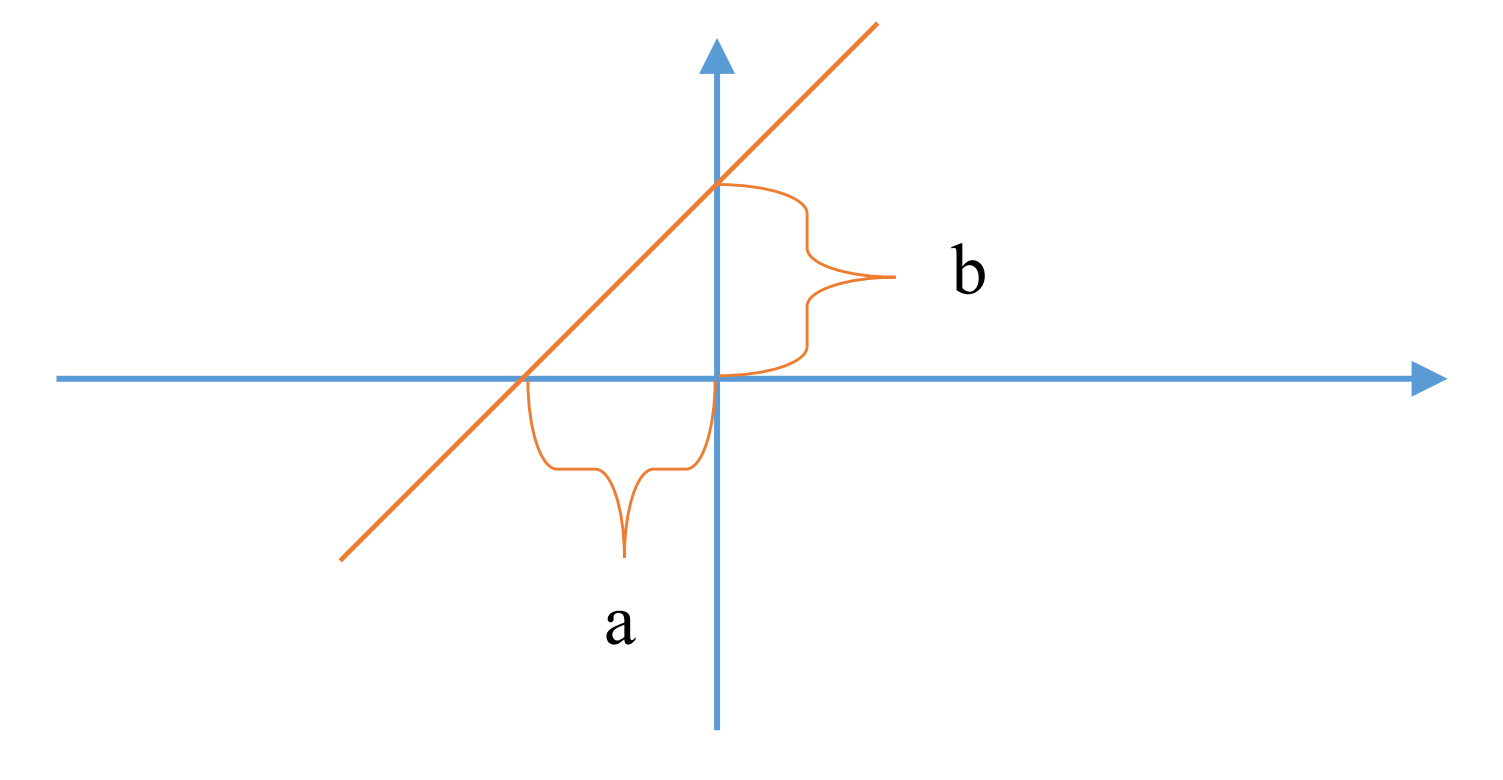
\includegraphics[scale=0.3]{images/dpsk3_1.png}\end{center}





\section{Нормальное уравнение прямой.}
Рассмотрим некоторую прямую $\Delta$. Построим прямую $\Delta_2$, проходящую через начало координат и перпендикулярную прямой $\Delta$. Пусть $P$ --- точка пересечения прямых $\Delta$ и $\Delta_2$. Обозначим через $n$ единичный вектор, перпендикулярный прямой $\Delta$ и сонаправленный с вектором $\overrightarrow{OP}$. \\\\
\begin{center}
	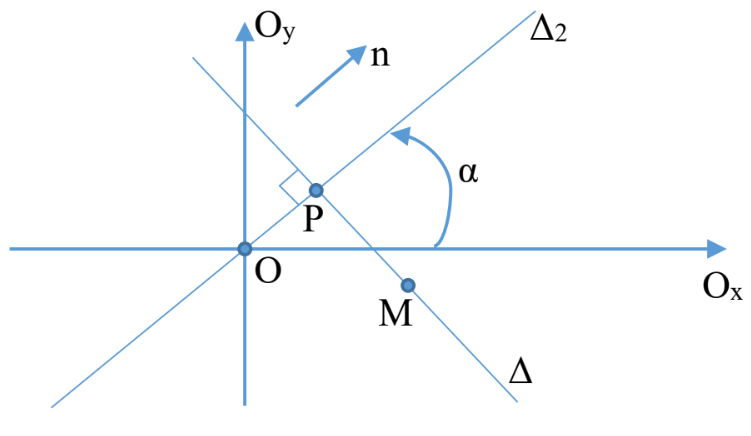
\includegraphics[scale=0.4]{images/pic3_2.png}
\end{center}
Если точки $O$ и $P$ совпадают, то $n$ --- произвольный единичный вектор, перпендикулярный прямой $\Delta$. Обозначим через $p$ расстояние между точками $O$ и $P$, то есть $p$ = $|\overline{OP}|$. Через $\alpha$ обозначим угол, на который надо повернуть ось $Ox$ против часовой стрелки, чтобы ее направление совпало с направлением нормального вектора $n$. Тогда вектор $n$ имеет координаты $n(cos \alpha, cos \beta)$. \\\\
Пусть $M(x, y)$ --- произвольная точка плоскости. $M\in\Delta\Longleftrightarrow\overrightarrow{PM}\perp n\Longleftrightarrow\overrightarrow{PM}\cdot n = 0.$ \\\\
По определению суммы векторов $\overrightarrow{PM} = \overrightarrow{PO} + \overrightarrow{OM} = \overrightarrow{OM} - \overrightarrow{OP}$, тогда подставим и получим $(\overrightarrow{OM} - \overrightarrow{OP})\cdot n = 0 \Rightarrow \overrightarrow{OM} \cdot n - \overrightarrow{OP} \cdot n = 0.$ Распишем уменьшаемое и вычитаемое: \\
$\overrightarrow{OM}\cdot n = (x, y)\cdot (cos \alpha, sin \alpha) = x cos \alpha + y sin \alpha$.\\
$\overrightarrow{OP}\cdot n = |\overline{OP}| \cdot |n| \cdot cos \underset{=0}{(\overrightarrow{OP}, n)} = p \cdot 1 \cdot 1 = p \Rightarrow$ получаем уравнение $$xcos \alpha + ysin \alpha - p = 0.\eqno(3.2.1)$$
$\bullet$\textit{Уравнение $(3.2.1)$ называется нормальным \textbf{нормальным уравнением прямой}}.\\\\
Пусть $M_0(x_0, y_0)$ --- произвольная точка плоскости, а точка $M_1(x_1, y_1)$ --- ее проекция на прямую $\Delta$. Обозначим через $\rho(M_0, \Delta)$ --- расстояние от точки $M_0$ до прямой $\Delta$. Тогда $\rho(M_0, \Delta)$ = $| \overline{M_1 M_0} |$. \\\\
$\bullet$ \textit{\textbf{Отклонением} точки $M_0$ от прямой $\Delta$ называется число} $\delta(M_0, \Delta) = \begin{cases} \rho(M_0, \Delta), \ \overrightarrow{M_1 M_0} \uparrow\uparrow n, \\ -\rho(M_0, \Delta), \ \overrightarrow{M_1 M_0} \uparrow\downarrow n. \end{cases}$ \\\\
Из определения отклонения следует, что $\rho(M_0,\Delta) = |\delta(M_0,\Delta)|$ и $\delta(M_0, \Delta) = \text{ПР}_n$ $\overrightarrow{M_1 M_0}$.
\newtheorem*{t4_2_1}{Теорема}\begin{t4_2_1} Если $xcos \alpha + ysin \alpha - p = 0$ --- нормальное уравнение прямой, то отклонение точки $M_0(x_0, y_0)$ от прямой $\Delta$ следующее: $\delta(M_0, \Delta)$ = $x_0 cos \alpha + y_0 sin \alpha - p$. \end{t4_2_1}
\begin{Proof}
	$\delta(M_0, \Delta) = \text{ПР}_n \overrightarrow{M_1 M_0} =\ [\ \overrightarrow{M_1 M_0} = \overrightarrow{M_1 O} + \overrightarrow{O M_0} = \overrightarrow{O M_0} - \overrightarrow{O M_1} \ ]\ \Rightarrow \text{ПР}_n (\overrightarrow{O M_0} - \overrightarrow{O M_1}) = \\ = \text{ПР}_n \overrightarrow{O M_0} - \text{ПР}_n \overrightarrow{O M_1}.$ Распишем обе проекции по отдельности:\\\\
	$\text{ПР}_n \overrightarrow{O M_0} = |\overrightarrow{O M_0}| \cdot cos (n, \overrightarrow{O M_0}) \cdot 1 = \overrightarrow{O M_0} \cdot n = (x_0, y_0)(cos \alpha, sin \alpha) = x_0 cos \alpha + y_0 sin \alpha$. \\\\
	$\text{ПР}_n \overrightarrow{O M_1} = p$ (по определению величины проекции). Тогда, подставив вместо проекций полученные выражения, имеем $\delta(M_0, \Delta)=\text{ПР}_n \overrightarrow{O M_0} - \text{ПР}_n \overrightarrow{O M_1} = x_0 cos \alpha + y_0 sin\alpha - p$.
\end{Proof}\\\\
Построим нормальное уравнение прямой с помощью общего уравнения.\\
Пусть прямая  $\Delta$ удовлетворяет общему уравнению $$Ax + By + C = 0.\eqno (3.2.2)$$
И пусть уравнение (3.2.1) --- нормальное уравнение прямой $\Delta$.
Так как уравнения эти уравнения определяют одну прямую, то их коэффициенты пропорциональны, то есть $\exists\lambda\in\mathbb{R}$, $cos \alpha$ = $\lambda\cdot A$, $sin \alpha$ = $\lambda\cdot B$, $-p$ = $\lambda\cdot C$.
Из первых двух равенств имеем $1 = cos^2 \alpha + sin^2 \alpha = \lambda ^2 (A^2 + B^2)$ $\Rightarrow$ $\lambda$ = $\pm$ $\dfrac{1}{\sqrt{A^2 + B^2}}$, причем из полученного соотношения следует, что знак $\lambda$ противоположен знаку $C$.\\\\ 
$\bullet$ \textit{Полученное таким образом число $\lambda$ называется \textbf{нормирующим множителем} для общего уравнения $(3.2.2)$, так как, домножив это уравнение на $\lambda$, получим нормальное уравнение.}


\section{Параметрическое и каноническое уравнения прямой. Уравнение прямой с угловым коэффициентом.}
До этого мы задавали прямую с помощью нормального вектора. Теперь зададим её другим способом.\\\\
$\bullet$ \textit{Ненулевой вектор, параллельный прямой, называется \textbf{направляющим вектором} прямой.} \\\\
Рассмотрим некоторую прямую $\Delta$ и пусть $a(a_1, a_2)$ --- ее направляющий вектор, $M_0 (x_0, y_0)$ --- точка на прямой. Тогда точка $M (x, y)$ $\in$ $\Delta$ $\Longleftrightarrow$ $\overrightarrow{M_0 M}$ $\parallel$ $a$.
\begin{center}
	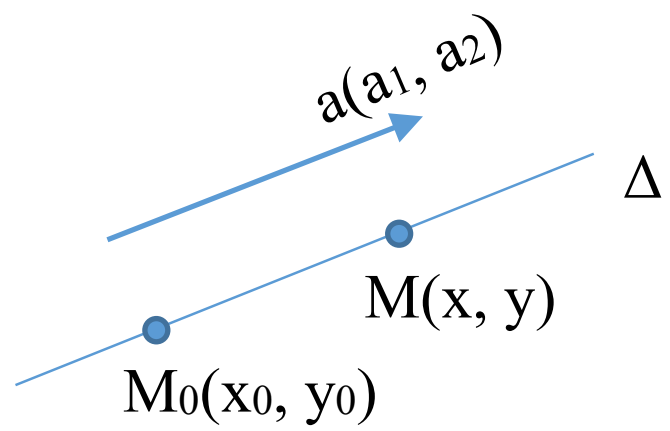
\includegraphics[scale=0.3]{images/line4_3.png}
\end{center}
Следовательно, $\exists$$t$ $\in$ $R$ такое, что $\overrightarrow{M_0 M}$ = $ta$. 
$\overrightarrow{M_0 M}$ = $\overrightarrow{M_0 O}$ + $\overrightarrow{O M}$ = $\overrightarrow{O M}$ - $\overrightarrow{O M_0}$ = $r_m - r_{m_0}$. Получаем $r_m - r_{m_0}$ = $ta$. Тогда
$$r_m = r_{m_0} + ta\eqno(3.3.1)$$
$\bullet$ \textit{Уравнение $(3.3.1)$ называется \textbf{параметрическим уравнением в векторной форме}.}  \\\\
Запишем это уравнение через координаты:
$$\begin{cases}
	x = x_0 + t\cdot a_1,\\
	y = y_0 + t\cdot a_2. 
\end{cases}\eqno(3.3.2)$$
$\bullet$ \textit{Уравнение $(3.3.2)$ называется \textbf{параметрическим уравнением прямой в координатной форме}}. \\\\	
Если прямая не параллельна ни одной из координатных осей, то $a_1$ $\not=$ $0$ и $a_2$ $\not=$ $0$.\\ Тогда $t$ = $\dfrac{x - x_0}{a_1}$, $t$ = $\dfrac{y - y_0}{a_2}$ $\Rightarrow$ $$\dfrac{x - x_0}{a_1} = \dfrac{y - y_0}{a_2}.\eqno(3.3.3)$$
$\bullet$ \textit{Уравнение $(3.3.3)$ называется \textbf{каноническим уравнением прямой}}. \\\\
Если прямая параллельна одной из координатных осей, то уравнение прямой также может быть записано в каноническом виде. При этом равенство нулю в знаменателе означает не деление на нуль, а равенство нулю числителя для всех точек прямой.
Рассмотрим прямую, изображенную на графике:
\begin{center}
	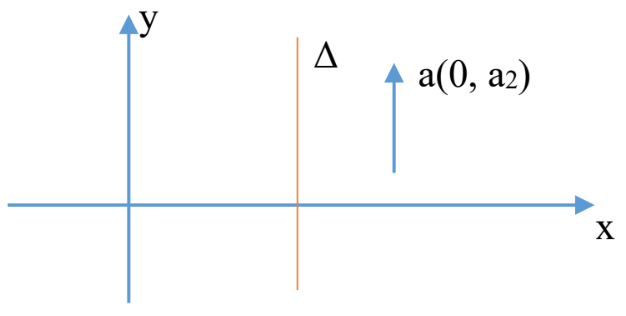
\includegraphics[scale=0.4]{images/dpsk4_3.png}
\end{center}
Ее параметрическое уравнение имеет вид:	$\begin{cases}
	x = x_0, \\
	y = y_0 + a_2 \cdot t.
\end{cases}$\\
Тогда каноническое уравнение этой прямой имеет вид:
$\dfrac{x - x_0}{0} = \dfrac{y - y_0}{a_2}$.\\\\
Если прямая $\Delta$ проходит через две различные точки $M_0 (x_0, y_0)$ и $M_1 (x_1, y_1)$, то в качестве направляющего вектора прямой можно взять вектор $\overrightarrow{M_0 M_1}$ $(x_1 - x_0, y_1 - y_0)$. Тогда уравнение прямой примет вид: $$\dfrac{x - x_0}{x_1 - x_0} = \dfrac{y - y_0}{y_1 - y_0}.\eqno(3.3.4)$$
$\bullet$ \textit{Уравнение $(3.3.4)$ называется \textbf{уравнением прямой, проходящей через 2 точки}.} \\\\
Пусть прямая $\Delta$ не параллельна оси $Oy$, и пусть $a(a_1, a_2)$ --- ее направляющий вектор ($a_1$ $\not=$ 0) и точка $M_0 (x_0, y_0)$ $\in$ $\Delta$. \\\\
$\bullet$ \textit{\textbf{Углом наклона прямой} $\Delta$ к оси $Ox$ называется угол, на который необходимо повернуть ось $Ox$ против часовой стрелки, чтобы она стала параллельна прямой $\Delta$.} \\\\
$\bullet$ \textit{Тангенс угла наклона прямой к оси $Ox$ называется \textbf{угловым коэффициентом прямой}}. \\\\
То есть если $\varphi$ --- угол наклона, а $k$ --- угловой коэффициент, то $k = tg \varphi$. \\
\newtheorem*{t4_3_1}{Теорема}\begin{t4_3_1} Если вектор $a(a_1, a_2)$ --- направляющий вектор прямой $\Delta$, то $k$ = $\dfrac{a_2}{a_1}$. \end{t4_3_1}
\begin{Proof}
	\begin{enumerate}
		\item Пусть направляющий вектор $a$ прямой $\Delta$ направлен так, что $\angle(a, i)$ = $\varphi$.
		Тогда\\ $a_1$ = ПР$_{Ox}$$a$ = ПР$_i$$a$ = $|a|\cdot cos(a, i)$ = $|a|\cdot cos \varphi$.\\
		$a_2$ = ПР$_{Oy}$$a$ = ПР$_j$$a$ = $|a|\cdot cos(a, j)$ = $|a|\cdot cos (\pm (\dfrac{\pi}{2} - \varphi))$ = $|a|\cdot sin \varphi$. \\
		Тогда $\dfrac{a_2}{a_1}$ = $\dfrac{|a|\cdot sin \varphi}{|a|\cdot cos \varphi}$ = $tg \varphi$ = $k$.
		\item Пусть вектор $a$ направлен так, что $\angle$$(a, i)$ $\not=$ $\varphi$. Тогда вектор $b = -a$ также является направляющим вектором и $\angle$$(b, i)$ = $\varphi$. По доказанному выше, $k = \dfrac{b_2}{b_1} = \dfrac{-a_2}{-a_1} = \dfrac{a_2}{a_1}$.
	\end{enumerate}
\end{Proof}\\
Пусть $\dfrac{x - x_0}{a_1} = \dfrac{y - y_0}{a_2}$ --- каноническое уравнение прямой $\Delta$. Тогда, домножим все на $a_2$ и получим $y - y_0$ = $\dfrac{a_2}{a_1}$$(x - x_0)$ = $k (x - x_0)$ $\Rightarrow$ $$y - y_0 = k (x - x_0).\eqno(3.3.5)$$ $\bullet$ \textit{Уравнение $(3.3.5)$ называется \textbf{уравнением с угловым коэффициентом прямой, проходящей через точку с координатами $(x_0, y_0)$}}. \\\\
Обозначим $b$ = $y_0 - kx_0$. Тогда уравнение прямой имеет вид $$y = kx + b.\eqno(3.3.6)$$
$\bullet$ \textit{Уравнение $(3.3.6)$ называется \textbf{уравнением прямой с угловым коэффициентом}}. \\\\






\chapter{Уравнения плоскости и прямой в пространстве}

\section{Уравнение плоскости.}
$\bullet$ \textit{\textbf{Нормальным вектором плоскости} называется ненулевой вектор, перпендикулярный плоскости.} \\\\
Рассмотрим некоторую плоскость П, проходящую через точку $M_0 (x_0, y_0, z_0)$ перпендикулярно вектору $n(A, B, C).$
\begin{center}
	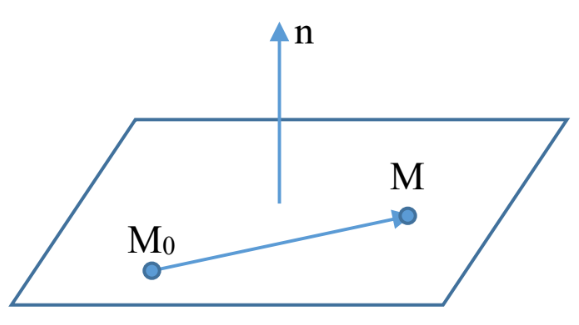
\includegraphics[scale=0.4]{images/pl4_1.png}
\end{center} Точка $M(x, y, z)$ $\in$ П $\Longleftrightarrow$ $\overrightarrow{M_0 M}$ $\perp$ $n$ $\Longleftrightarrow$ $\overrightarrow{M_0 M}$ $\cdot$ $n$ = $0$.
Таким образом получаем уравнение
$$A(x - x_0) + B(y - y_0) + C(z - z_0) = 0.\eqno(4.1.1)$$
$\bullet$ \textit{Уравнение $(4.1.1)$ называется \textbf{уравнением плоскости, проходящей через точку $M_0(x_0, y_0, z_0)$ перпендикулярно вектору $n(A, B,C)$}}. \\\\
Обозначим $D = -A x_0 - B y_0 - C z_0$, тогда уравнение (4.1.1) примет вид \\
$$Ax + By + Cz + D = 0\quad A^2 + B^2 + C^2 \not = 0.\eqno(4.1.2)$$ $\bullet$ \textit{Уравнение $(4.1.2)$ называется \textbf{общим уравнением плоскости}}.
\newtheorem*{t5_1_1}{Теорема}\begin{t5_1_1} Любая плоскость в пространстве может быть задана уравнением вида $(4.1.2)$. Любое уравнение вида $(4.1.2)$ определяет плоскость. \end{t5_1_1}\begin{Proof}
	Доказательство аналогично подобной теореме для случая с прямой.
\end{Proof} 
\newtheorem*{t5_1_2}{Теорема}\begin{t5_1_2} Если два общих уравнения $\begin{matrix} A_1 x + B_1 y + C_1 z + D_1 = 0, \\ A_2 x + B_2 y + C_2 z + D_2 = 0 \end{matrix}$ определяют одну плоскость, то существует действительное число $\lambda$ такое, что \begin{center}
		$A_1 = \lambda A_2$, $B_1 = \lambda B_2$, $C_1 = \lambda C_2$, $D_1 = \lambda D_2$. 
	\end{center} 
\end{t5_1_2} \begin{Proof}
	Доказательство аналогично подобной теореме для случая с прямой.
\end{Proof}\\\\
Пусть даны два нормальных вектора $n_1(A_1, B_1, C_1)$ и $n_2(A_2, B_2, C_2)$. Тогда косинус угла между плоскостями равен косинусу угла между нормальными векторами к плоскостям:
$$cos(n_1, n_2) = \dfrac{n_1 \cdot n_2}{|n_1| \cdot |n_2|}.$$
$\bullet$ \textit{Общее уравнение плоскости называется \textbf{полным}, если все его коэффициенты отличны от нуля, в противном случае называется \textbf{неполным}}. \\\\
Неполные уравнения описывают плоскости, параллельные координатным осям и (или) проходящие через начало координат.\\\\
Пусть $Ax + By + Cz + D = 0$ --- полное общее уравнение плоскости. Перенесем $D$ с противоположным знаком в правую часть уравнения и разделим на него же. Тогда получим
\begin{center}
	$\dfrac{Ax}{-D}$ + $\dfrac{By}{-D}$ + $\dfrac{Cz}{-D}$ = 1 $\Rightarrow$ $\dfrac{x}{\dfrac{-D}{A}}$ + $\dfrac{y}{\dfrac{-D}{B}}$ + $\dfrac{z}{\dfrac{-D}{C}}$ = 1 $\Rightarrow$ $\Big[\dfrac{-D}{A} = a, \dfrac{-D}{B} = b, \dfrac{-D}{C} = c\Big]$ $\Rightarrow$ $$\dfrac{x}{a} + \dfrac{y}{b} + \dfrac{z}{c} = 1.\eqno(4.1.3)$$
\end{center}
$\bullet$ \textit{Уравнение $(4.1.3)$ называется \textbf{уравнением плоскости в отрезках}}.\\\\
Числа $a, b, c$ являются величинами направленных отрезков, отсекаемых плоскостью по координатным осям от начала координат. \\\\
Пусть П --- произвольная плоскость. Построим прямую $\Delta$, проходящую через начало координат перпендикулярно плоскости П. Обозначим через $P$ точку пересечения прямой $\Delta$ и плоскости П. Через $p$ обозначим $|\overline{OP}|$, а через $n$ --- единичный вектор, перпендикулярный плоскости П и сонаправленный с вектором $\overrightarrow{OP}.$ Если точки $O$ и $P$ совпадают, то направление единичного нормального вектора $n$ выбираем произвольно. \begin{center}
	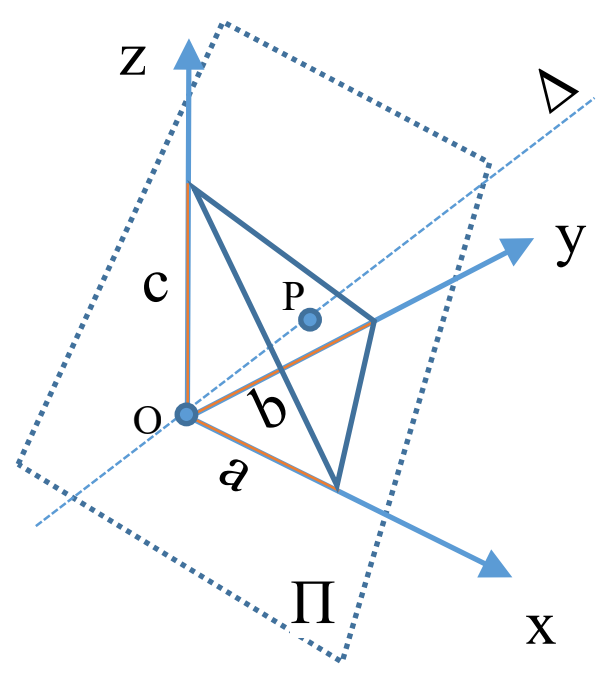
\includegraphics[scale=0.3]{images/pl2_4_1.png}
\end{center}
Так как $n$ --- единичный вектор, то его координаты $n(cos \alpha, cos \beta, cos \gamma)$, где $\alpha$, $\beta$, $\gamma$ --- углы между $n$ и осями координат $Ox, Oy, Oz$ соответственно. \\\\
Точка $M(x, y, z)$ $\in$ П $\Longleftrightarrow$ $x\cdot cos \alpha + y \cdot cos \beta + z \cdot cos \gamma = p$. Перенесем $p$ в левую сторону и получим $$x\cdot cos \alpha + y \cdot cos \beta + z \cdot cos \gamma - p = 0.\eqno(4.1.4)$$ $\bullet$ \textit{Уравнение $(4.1.4)$ называется \textbf{нормальным уравнением плоскости}}. \\\\
Нормальное уравнение можно построить из общего уравнения, домножив его на нормирующий множитель
$\lambda$ = $\pm$ $\dfrac{1}{\sqrt{A^2 + B^2 + C^2}}$, где знак $\lambda$ противоположен знаку $D$.\\\\
Пусть $M(x, y, z)$ --- некоторая произвольная точка пространства, $M_1$ --- ее проекция на плоскость П,  тогда $\rho(M, \text{П}) = | \overline{M_1 M} |$ --- расстояние от точки $M$ до плоскости П. \\\\
$\bullet$ \textit{\textbf{Отклонением} $\delta(M, \text{П})$ называется число, равное}
$\delta(M, \text{П}) = \begin{cases} \rho(M, \text{П}), \overrightarrow{M_1 M} \uparrow\uparrow n, \\ -\rho(M, \text{П}), \overrightarrow{M_1 M} \uparrow\downarrow n. \end{cases}$
\newtheorem*{t5_1_3}{Теорема} \begin{t5_1_3} Если $x\cdot cos\alpha + y\cdot cos\beta + z\cdot cos\gamma - p = 0$ --- нормальное уравнение плоскости П, то отклонение точки $M_0(x_0, y_0, z_0)$ от плоскости П равняется:$$\delta(M_0, \text{П}) = x_0 \cdot cos \alpha  +  y_0 \cdot cos \beta  +  z_0 \cdot cos \gamma  -  p.$$\end{t5_1_3}\begin{Proof}
	Доказательство аналогично подобной теореме для случая с прямой.
\end{Proof}\\\\
Заметим, что $\rho(M_0, $П$) = |x_0\cdot cos\alpha + y_0 \cdot cos\beta + z_0\cdot cos\gamma - p|$.\\\\
Пусть плоскость П проходит через точку $M_0(x_0, y_0, z_0)$ параллельно двум неколлинеарным векторам $a(a_1, a_2, a_3)$ и $b(b_1, b_2, b_3)$. \begin{center}
	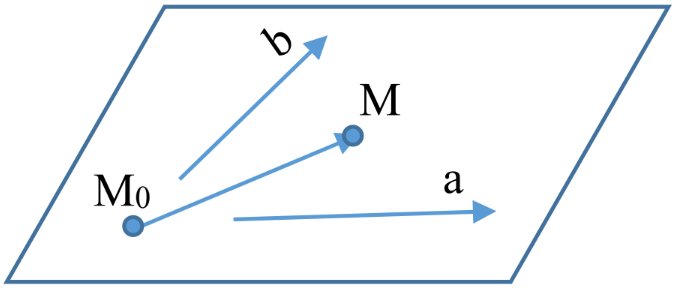
\includegraphics[scale=0.35]{images/pl3_4_1.png}
\end{center}
Тогда $M(x, y, z)$ $\in$ П $\Longleftrightarrow$ $\overrightarrow{M_0 M}$, $a, b$ --- компланарные $\Longleftrightarrow$ $\overrightarrow{M_0 M}$ $\cdot$ $a$ $\cdot$ $b$ = 0  $\Longleftrightarrow$ $$(r_m - r_{m_0}) \cdot a \cdot b = 0.\eqno(4.1.5)$$  $\bullet$ \textit{Уранвнение $(4.1.5)$ называется \textbf{уравнением плоскости, проходящей через точку $M_0$, параллельно неколлениарным векторам $a$ и $b$ в векторной форме}}. \\\\
Так же это уравнение можно записать через определитель:
$$\begin{vmatrix} x - x_0 && y - y_0 && z - z_0 \\ a_1 && a_2 && a_3 \\ b_1 && b_2 && b_3 \end{vmatrix} = 0.\eqno(4.1.6)$$ 
$\bullet$ \textit{Уравнение $(4.1.6)$ называется \textbf{уравнением плоскости, проходящей через точку $M_0$, параллельно неколлениарным векторам $a$ и $b$}}.\\\\
Если плоскость П проходит через три точки, не лежащие на одной прямой $M_0(x_0, y_0, z_0)$, $M_1(x_1, y_1, z_1)$, $M_2(x_2, y_2, z_2)$, то в качестве неколлинеарных векторов, параллельных плоскости, можно взять $\overrightarrow{M_0 M}$ и $\overrightarrow{M_0 M_2}$ и тогда уравнение примет вид:
$$\begin{vmatrix} x - x_0 && y - y_0 && z - z_0 \\ x_1 - x_0 && y_1 - y_0 && z_1 - z_0 \\ x_2 - x_0 && y_2 - y_0 && z_2 - z_0  \end{vmatrix} = 0.\eqno(4.1.7)$$
$\bullet$ \textit{Уравнение $(4.1.7)$ называется \textbf{уравнением плоскости, проходящей через три точки}}.\\\\
Так как векторы $a$ и $b$ неколлинеарны, то они на плоскости П образуют базис. Следовательно, любой вектор, параллельный плоскости, в том числе и $\overrightarrow{M_0 M}$, если точка $M$ принадлежит плоскости П, может быть разложен по этому базису, то есть представим в виде $\overrightarrow{M_0 M} = t \cdot a + s \cdot b$, где $t, s$ $\in$ $\mathbb{R}$. Тогда
$$r_m = r_{m_0} + t \cdot a + s \cdot b.\eqno(4.1.8)$$
$\bullet$ \textit{Уравнение $(4.1.8)$ называется \textbf{параметрическим уравнением плоскости в векторной форме}}.\\\\
Распишем векторы по координатам и получим
$$\begin{cases}
	x = x_0 + t \cdot a_1 + s \cdot b_1, \\
	y = y_0 + t \cdot a_2 + s \cdot b_2, \\
	z = z_0 + t \cdot a_3 + s \cdot b_3.
\end{cases}\eqno(4.1.9)$$
$\bullet$ \textit{Уравнение $(4.1.9)$ называется \textbf{параметрическим уравнением плоскости в координатной форме}}.







\section{Уравнение прямой в пространстве.}
$\bullet$ \textit{Ненулевой вектор, параллельный прямой, называется \textbf{направляющим вектором} прямой.} \\\\
Рассмотрим некоторую прямую $\Delta$ и пусть $a(a_1, a_2, a_3)$ --- ее направляющий вектор, \\ $M_0(x_0, y_0, z_0)$ --- точка на прямой $\Delta$. Тогда точка $M(x, y, z)$ $\in$ $\Delta$ $\Longleftrightarrow$ $\overrightarrow{M_0 M}$ $\parallel$ $a$ $\Longleftrightarrow$ \\$\exists$$t$ $\in$ $\mathbb{R}$ :  $\overrightarrow{M_0 M}$ = $t \cdot a$. Отсюда получаем \\
$$r_m = r_{m_0} + t \cdot a.\eqno(4.2.1)$$ $\bullet$ \textit{Уравнение $(4.2.1)$ называется \textbf{параметрическим уравнением прямой в векторной форме}}. \\\\
Распишем это уравнения через координаты векторов и получим
$$\begin{cases}
	x = x_0 + t \cdot a_1,\\
	y = y_0 + t \cdot a_2, \\
	z = z_0 + t \cdot a_3.
\end{cases}\eqno(4.2.2)$$
$\bullet$ \textit{Уравнение $(4.2.2)$ называется \textbf{параметрическим уравнением прямой в координатной форме}}. \\\\
Выразив параметр $t$ из каждого параметрического уравнения получим
$$\dfrac{x - x_0}{a_1} = \dfrac{y - y_0}{a_2} = \dfrac{z - z_0}{a_3}.\eqno(4.2.3)$$ 
$\bullet$ \textit{Уравнение $(4.2.3)$ называется \textbf{каноническим уравнением прямой}}.\\\\
Если прямая $\Delta$ проходит через две различные точки $M_0(x_0, y_0, z_0)$ и $M_1(x_1, y_1, z_1)$, то в качестве направляющего вектора можно взять вектор $\overrightarrow{M_0 M_1}$. Подставляем координаты в каноническое уравнение и получаем
$$\dfrac{x - x_0}{x_1 - x_0} = \dfrac{y - y_0}{y_1 - y_0} = \dfrac{z - z_0}{z_1 - z_0}.\eqno(4.2.4)$$ $\bullet$ \textit{Уравнение $(4.2.4)$ называется \textbf{уравнением прямой по двум точкам}}. \\\\
Пусть $A_1 x + B_1 y + C_1 z + D_1 = 0$ и $A_2 x + B_2 y + C_2 z + D_2 = 0$ --- две различные плоскости, проходящие через прямую $\Delta$, тогда точка $M(x, y, z)$ $\in$ $\Delta$ $\Longleftrightarrow$ ее координаты удовлетворяют каждому уравнению плоскости. Следовательно, \\\\
$$\begin{cases}
	A_1 x + B_1 y + C_1 z + D_1 = 0, \\
	A_2 x + B_2 y + C_2 z + D_2 = 0. \\ \end{cases}\eqno(4.2.5)$$
$\bullet$ \textit{Уравнение $(4.2.5)$ называется \textbf{уравнением прямой, заданной как линия пересечения двух плоскостей (общим уравнением прямой)}}.\\\\
Рассмотрим взаимное расположение прямых в пространстве. Возьмём две прямые $\Delta_1$ и $\Delta_2$, проходящие через точки $M_0$ и $M_1$, описанные каноническими уравненениями $\dfrac{x - x_0}{a_1}$ = $\dfrac{y - y_0}{a_2}$ = $\dfrac{z - z_0}{a_3}$ и $\dfrac{x - x_1}{b_1}$ = $\dfrac{y - y_1}{b_2}$ = $\dfrac{z - z_1}{b_3}$ соответственно. При этом $a(a_1, a_2, a_3)$ и $b(b_1, b_2, b_3)$ --- два направляющих вектора соответственно.
\begin{enumerate}
	\item прямые совпадают, если $a$ $\parallel$ $b$ $\parallel$ $\overrightarrow{M_0 M_1}$ $\Rightarrow$ $\dfrac{a_1}{b_1}$ = $\dfrac{a_2}{b_2}$ = $\dfrac{a_3}{b_3}$;
	\item прямые параллельны, если $a$ $\parallel$ $b$, $\overrightarrow{M_0 M_1}$ $\nparallel$ $a, b$;
	\item прямые пересекаются, если $a$ $\nparallel$ $b$ $\nparallel$ $\overrightarrow{M_0 M_1}$, но при этом $\overrightarrow{M_0 M_1}\cdot a \cdot b = 0$ (то есть векторы $a, b, \overrightarrow{M_0 M_1}$ компланарны);
	\item прямые скрещивающиеся, если $a$ $\nparallel$ $b$ $\nparallel$ $\overrightarrow{M_0 M_1}$, но при этом $\overrightarrow{M_0 M_1}\cdot a \cdot b \not= 0$ (то есть $a, b, \overrightarrow{M_0 M_1}$ не компланарны).
\end{enumerate}
\begin{center}
	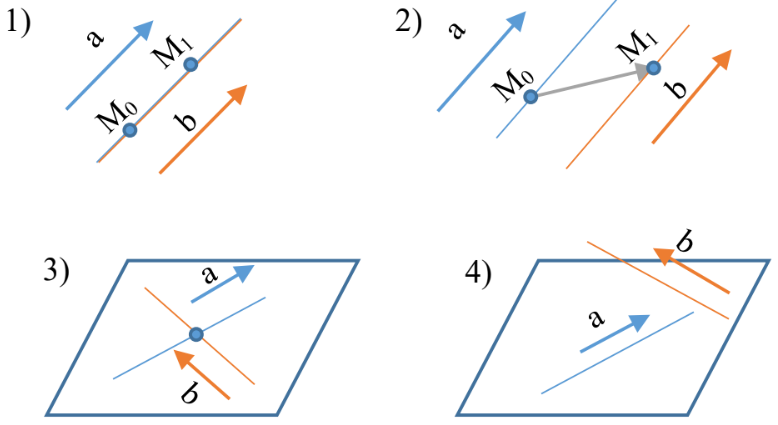
\includegraphics[scale=0.4]{images/cases5_1.png}
\end{center}
Заметим, что угол между двумя прямыми равен углу между их направляющими векторами, то есть
\begin{center}
	$cos(\Delta_1, \Delta_2) = \dfrac{|a \cdot b|}{|a| \cdot |b|}.$
\end{center}
Рассмотрим взаимное расположение прямой и плоскости. Пусть прямая задана каноническим уравнением $\dfrac{x - x_0}{a_1}$ = $\dfrac{y - y_0}{a_2}$ = $\dfrac{z - z_0}{a_3}$, а плоскость задана общим уравнением $Ax + By + Cz + D = 0$.
\begin{enumerate}
	\item Если прямая лежит на плоскости, то $a$ $\perp$ $n$ $\Longleftrightarrow$ $a \cdot n$ = 0, а сами прямая и плоскость имеют одну общую точку.
	\item Прямая параллельна плоскости, если $a \cdot n$ = 0, а общих точек у них нет.
	\item Прямая и плоскость пересекаются, если $a \cdot n$ $\not=$ 0.
\end{enumerate}
\begin{center}
	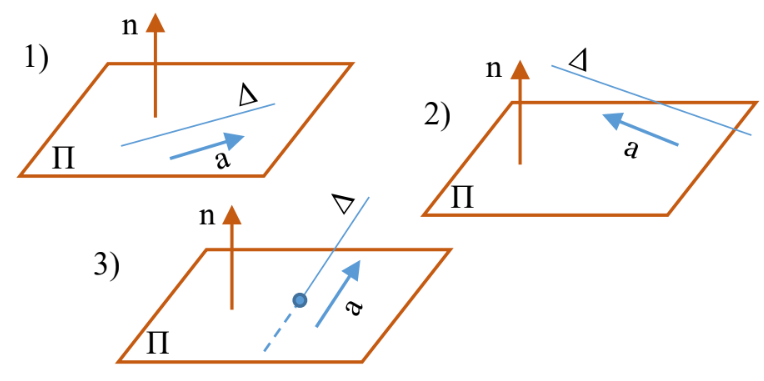
\includegraphics[scale=0.4]{images/cases2_5_2.png}
\end{center}
При этом угол между прямой и плоскостью равен углу между нормальным вектором плоскости и направляющим вектором прямой. 
\begin{center}
	$sin(\Delta, \text{П}) = \dfrac{|a \cdot n|}{|a| \cdot |n|}$.
\end{center}




\chapter{Линии и поверхности второго порядка}


\section{Эллипс.}
$\bullet$ \textit{\textbf{Эллипсом} называется множество всех точек плоскости,
	cумма расстояний от которых до данных двух точек $F_1$ и $F_2$
	есть величина постоянная. При этом точки $F_1$ и $F_2$
	называются \textbf{фокусами эллипса}}.
\begin{center}
	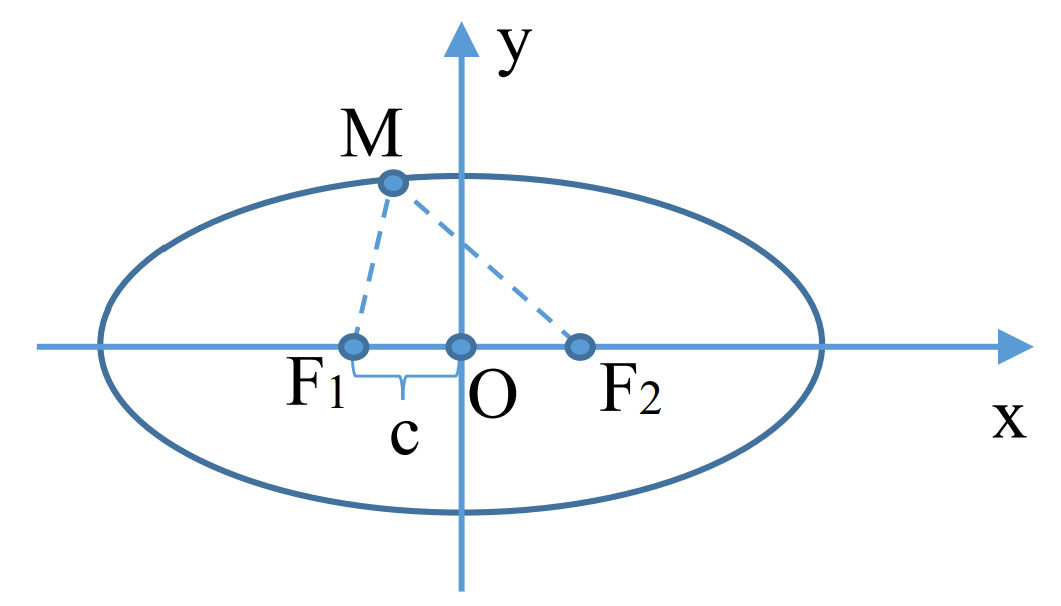
\includegraphics[scale=0.4]{images/ellipse.png}
\end{center}
Выведем формулу: пусть $F_1$ и $F_2$ – фокусы, $|\overline{F_1F_2}| = 2c.$\\\\
Построим ДПСК, чтобы $Ox$ проходила через фокусы так, чтобы направление вектора $\overrightarrow{F_1F_2}$ совпадало с
направлением оси $x$, а начало координат располагалось в центе $\overline{F_1F_2}$. Тогда фокусы $F_1$ и $F_2$ имеют
координаты $(-c, 0)$ и $(c, 0)$ соответственно. И пусть $2a$ –-- сумма расстояний от точки эллипса $M(x, y)$
до фокусов. Заметим, что $2a > 2c \Rightarrow a > c$. Отрезки $MF_1$ и $MF_2$ назовём \textbf{фокальными радиусами точки $M$}. \\\\
По определению $|\overline{MF_1}| + |\overline{MF_2}| = 2a \Rightarrow$ $$\sqrt{(x + c)^2 + y^2} + \sqrt{(x - c)^2 + y^2} = 2a. \eqno(5.1.1)$$
Преобразуем уравнение $(5.1.1)$: $\sqrt{(x + c)^2 + y^2} = 2a - \sqrt{(x - c)^2 + y^2} \Leftrightarrow $  (возведём в квадрат)
$(x + c)^2 + y^2 = 4a^2 - 4a\sqrt{(x - c)^2 + y^2} + (x - c)^2 + y^2 \Leftrightarrow$ (перенесём выражение с корнем в левую
часть, всё остальное в правую и раскроем квадраты) $4a \sqrt{(x - c)^2 + y^2} = 4a^2 + x^2 + c^2 - 2xc - x^2 -
c^2 - 2xc + y^2 - y^2 \Leftrightarrow$ (уберём подобные) \\
$4a \sqrt{(x - c)^2 + y^2 = 4a^2 - 4xc} \Leftrightarrow$ (сократим на 4)
$a \sqrt{(x - c)^2 + y^2 = a2 - xc} \Leftrightarrow$ (снова возведём в квадрат) $a^2((x - c)^2 + y^2) = (a^2 - xc)^2 \Leftrightarrow$
(раскроем скобки) $a^2x^2 - 2a^2xc + a^2c^2 + a^2y^2 = a^4 - 2a^2xc + x^2c^2 \Leftrightarrow$ (сгруппируем $x$ и
$y$ слева, $a$ и $c$ справа и уберём подобные) $(a^2 - c^2)c^2 + a^2y^2 = a^2(a^2 - c^2)$.\\ Обозначим $b =
\sqrt{a^2 - c^2}$ (так как $a > c$). Заметим, что $b < a$. Тогда $b^2x^2 + a^2y^2 = a^2b^2$. \\Разделим обе части уравнения на
$a^2b^2$: $$\dfrac{x^2}{a^2} + \dfrac{y^2}{b^2} = 1.\eqno (5.1.2)$$
$\bullet$ \textit{Уравнение $(5.1.2)$ называется \textbf{каноническим уравнением эллипса}.}\\\\
Любая точка, удовлетворяющая уравнению $(5.1.1)$ (то есть принадлежащая эллипсу), удовлетворяет
уравнению $(5.1.2)$. Покажем, что любая точка, удовлетворяющая уравнению $(5.1.2)$, будет принадлежать
эллипсу.\\\\
Пусть $M_1(x_1, y_1)$ удовлетворяет $(5.1.2) \Rightarrow$ $$\dfrac{x_1^2}{a^2} + \dfrac{y_1^2}{b^2} = 1. \eqno(5.1.3)$$\\
$|\overline{M_1F_1}| = \sqrt{(x_1 + c)^2 + y^2} =$ [из $(5.1.3)\; y^2 = b^2(1 - \frac{x_1^2}{a^2})$] $=\sqrt{(x_1 + c)^2 + b^2(1 - \frac{x_1^2}{a^2})} = [b^2 = a^2 - c^2]=
\sqrt{(x_1 + c)^2 + (a^2 - c^2)(1 - \frac{x_1^2}{a^2})} = \sqrt{x_1^2 + 2x_1c + c^2 + a^2 = c^2 - x_1^2 + \frac{c^2x_1^2}{a^2}} = \sqrt{a^2 + 2x_1c + \frac{c^2x_1^2}{a^2}} = \sqrt{(a + \frac{c}{a}x_1)^2} = |a + \frac{c}{a}x_1|.$ Аналогично $|\overline{M_1F_2}| = |a - \frac{c}{a}x_1|.$ \\Раскроем модули, оценив подмодульные выражения. Из $(5.1.3)$ следует, что $\dfrac{x_1^2}{a^2} \leqslant 1 \Rightarrow -1 \leqslant \dfrac{x_1}{a} \leqslant 1
\Rightarrow -a < -c < \dfrac{cx_1}{a} < c < a \Rightarrow |a + \dfrac{c}{a}x_1| = a + \dfrac{c}{a}x_1,
|a - \dfrac{c}{a}x_1| = a - \dfrac{c}{a}x_1 \Rightarrow |\overline{M_1F_1}| + |\overline{M_1F_2}| = a + \dfrac{c}{a}x_1 + a - \dfrac{c}{a}x_1 = 2a \Rightarrow$ точка $M_1$ удовлетворяет уравнению $(5.1.1) \Rightarrow M_1$ --- точка, принадлежащая эллипсу
$\Rightarrow $ уравнение $(5.1.2)$ является каноническим уравнением эллипса, где $b<a.$\\\\
В случае, если $b>a$, каноническое уравнение имеет вид $\dfrac{x_1^2}{b^2} + \dfrac{y_1^2}{a^2} = 1$, а фокусы будут лежать не на $Ox$, а на $Oy$.\\\\
Исследование формы эллипса по его каноническому уравнению:\\\\
$\dfrac{x_1^2}{a^2}$ и $\dfrac{y_1^2}{b^2} \leqslant 1 \Rightarrow |x_1| \leqslant |a|$ и $|y_1| \leqslant |b|$, то есть эллипс --- линия ограниченная и расположенная внутри прямоугольника, которая ограничена прямыми $x = \pm a, y = \pm b$.
\begin{center}
	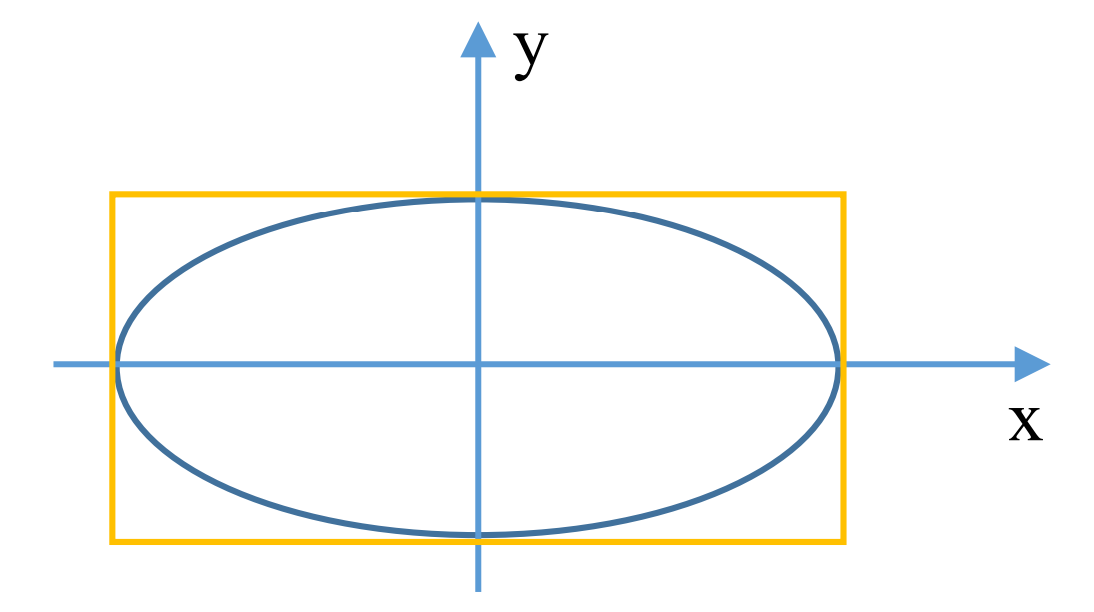
\includegraphics[scale=0.2]{images/ellipse_2.png}
\end{center}
В уравнении эллипса обе координаты имеют чётные степени, следовательно,
если точка $M_1(x, y)$ принадлежит эллипсу, то и точки $M_2(-x, y),
M_3(x, -y), M_4(-x, -y)$ также будут принадлежать эллипсу.\\\\
Эллипс симметричен относительно начала координат и осей.\\\\ $\bullet$ \textit{Центр симметрии называется \textbf{центром
		эллипса.}}\\\\
$\bullet$ \textit{Прямая, проходящая через фокусы, называется \textbf{большой осью эллипса}, перпендикулярная ей и
	проходящая через центр – \textbf{малая ось.} Точки пересечения осей эллипса с эллипсом ($Ox$ в точках
	$A_1(a, 0)$ и $A_2(-a, 0), Oy$ в точках $B_1(0, b)$ и $B_2(0, -b))$ называются \textbf{вершинами эллипса}. Отрезки $OA_1,OA_2, OB_1, OB_2$ – \textbf{полуоси} (большой и малой соответственно) эллипса с длинами $a$ и $b$.}\\\\
Рассмотрим поведение эллипса в первой четверти ДПСК: $\begin{cases}
	0 < x \leqslant a \\
	0 < y \leqslant b
\end{cases}$\\
$y = b \sqrt{1 - \frac{x^2}{a^2}}$ (из канонического уравнения) $\Rightarrow y=\dfrac{b}{a}(a^2 - x^2)^{\frac{1}{2}} \Rightarrow y' = \dfrac{b}{a}\cdot\dfrac{1}{2}(a^2 - x^2)^{-\frac{1}{2}}(-2x) = -\dfrac{b}{a}x(a^2 - x^2)^{-\frac{1}{2}} < 0$, то есть функция убывает. $y'' = - \dfrac{b}{a}\cdot\Big((a^2-x^2)^{-\frac{1}{2}}x + \dfrac{x(2x)(a^2-x^2)^{-\frac{3}{2}}}{2}\Big) = -\dfrac{ab}{(a^2-x^2)^{\frac{3}{2}}} < 0$, то есть график функции вогнут.

\section{Гипербола.}
$\bullet$ \textit{\textbf{Гиперболой} называется множество точек
	плоскости, модуль разности расстояний от
	которых до заранее заданных точек $F_1$ и $F_2$,
	называемых \textbf{фокусами гиперболы}, есть величина
	постоянная и меньшая, чем расстояние между фокусами.}. \begin{center}
	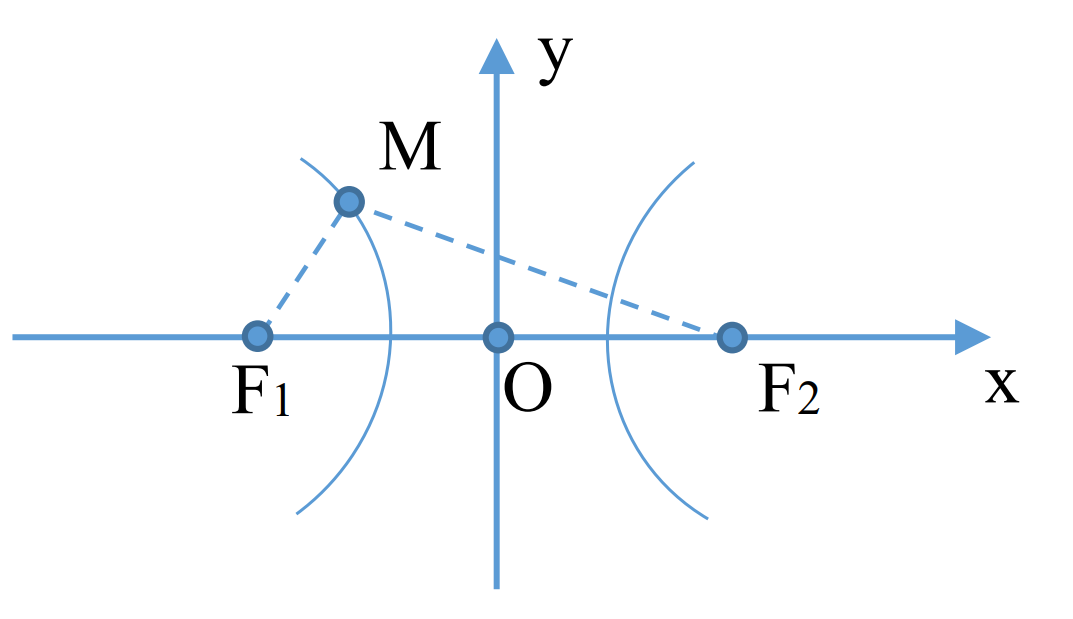
\includegraphics[scale=0.4]{images/gip1.png}
\end{center}
Выведем формулу: пусть $F_1$ и $F_2$ – фокусы, $|\overline{F_1F_2}| = 2c.$\\\\
Построим ДПСК: ось $Ox$ проходит через фокусы и соноправлена с $\overrightarrow{F_1F_2}$, а цент между фокусами --- начало координат. Обозначим модуль разности точек гиперболы до фокусов за $2a \Rightarrow 2a < 2c \Rightarrow a < c$.\\\\
Пусть $M(x, y)$ --- произвольная точка гиперболы. Как и в эллипсе, отрезки $MF_1$ и$ MF_2$ будем называть
фокальными радиусами.\\\\
По определению $||\overline{MF_1}| - |\overline{MF_2}|| = 2a \Rightarrow$ $$|\sqrt{(x+c)^2 + y^2} - \sqrt{(x-c)^2+ y^2}| = 2a.\eqno(5.2.1)$$
$\bullet$ \textit{Уравнение $(5.2.1)$ называется \textbf{уравнением гиперболы}.}\\\\
Преобразуем это уравнение. Раскроем модуль и получим: $\sqrt{(x+c)^2 + y^2} - \sqrt{(x-c)^2 +y^2} = \pm 2a \Leftrightarrow 
\sqrt{(x+c)^2+y^2} = \pm 2a + \sqrt{(x-c)^2 + y^2} \Leftrightarrow$ (возведём в квадрат и раскроем квадраты сумм и разности)
$x^2 + c^2 + 2xc + y^2 = 4a^2 + x^2 + c^2 - 2xc + y^2 \pm 4a\sqrt{(x-c)^2+y^2} \Leftrightarrow$ (приведём подобные)
$\pm a\sqrt{(x-c)^2 + y^2} = -a^2 + xc \Leftrightarrow$ (снова возведём в квадрат и раскроем квадраты сумм и разности) 
$a^2(x^2 + c^2 - 2xc + y^2) = a^4 + x^2c^2 - 2a^2xc \Leftrightarrow$ (снова приводим подобные, раскрыв скобку слева, после чего группируем по $x$ и $y$ справа, а без них слева)
$a^2(c^2-a^2) = x^2(c^2 - a^2) - a^2y^2$. Так как $c>a \Rightarrow c^2 - a^2 > 0 \Rightarrow$ обозначим $b = \sqrt{c^2 - a^2} \Rightarrow x^2b^2 - y^2a^2 = a^2b^2$.  $a$ и $b \ne 0 \Rightarrow$ делим на $a^2b^2$ и получаем $$\frac{x^2}{a^2} - \frac{y^2}{b^2} = 1. \eqno(5.2.2)$$\\\\
Любая точка, удовлетворяющая уравнению (5.2.1), то есть принадлежащая гиперболе, удовлетворяет и уравнению (5.2.2). Покажем,
что любая точка, удовлетворяющая уравнению (5.2.2), будет принадлежать гиперболе.\\\\
Пусть точка $M_1(x_1, y_1)$ удовлетворяет уравнению (5.2.2)$\Rightarrow$ $$\dfrac{x_1^2}{a^2} - \dfrac{y_1^2}{b^2} = 1.\eqno(5.2.3)$$ $|\overline{M_1F_1}| = \sqrt{(x_1 + c)^2 + y^2} = [$из (5.2.3) $y^2 = b^2(\dfrac{x_1^2}{a^2} - 1)] = \sqrt{(x_1 + c)^2 + b^2(\dfrac{x_1^2}{a^2} - 1)} =\\ \sqrt{(x_1 + c)^2 + (c^2 - a^2)(\dfrac{x_1^2}{a^2} - 1)} = \sqrt{x_1^2 + 2x_1c + c^2 + a^2 - c^2 - x_1^2 + \dfrac{c^2x_1^2}{a^2}} = \sqrt{(a + \dfrac{c}{a}x_1)^2} = |a+ \dfrac{c}{a}x_1|.$ Аналогично $|\overline{M_1F_2}| = |a - \dfrac{c}{a}x_1|$.\\
Из (5.2.3) следует, что $\dfrac{x_1^2}{a^2} \geqslant 1 \Rightarrow x_1 \geqslant a$ или $x_1 \leqslant -a$.\\\\
\begin{enumerate}
	\item Пусть $x_1 \geqslant a \Rightarrow \dfrac{cx_1}{a} > c > a \Rightarrow |\overline{M_1F_1}| = a + \dfrac{c}{a}x_1, |\overline{M_1F_2}| = -a + \dfrac{c}{a}x_1 \Rightarrow |\overline{M_1F_1}| - |\overline{M_1F_2}| = 2a$.
	\item  Пусть $x_1 \leqslant -a \Rightarrow \dfrac{cx_1}{a} < -c < -a < 0 \Rightarrow |\overline{M_1F_1}| = -a - \dfrac{c}{a}x_1, |\overline{M_1F_2}| = a - \dfrac{c}{a}x_1 \Rightarrow |\overline{M_1F_1}| - |\overline{M_1F_2}| = -2a \Rightarrow ||\overline{M_1F_1}| - |\overline{M_1F_2}|| = 2a$.
\end{enumerate} 
Следовательно, точка $M_1$ принадлежит гиперболе. Тогда\\\\ $\bullet$ \textit{Уравнение (5.2.2) называется \textbf{каноническим уравнением
		гиперболы}}.\\\\
Исследование формы гиперболы по её каноническому уравнению:\\\\
Из (5.2.2) следует, что $\dfrac{x_1^2}{a^2} \geqslant 1 \Rightarrow |x| \geqslant a \Rightarrow$ в полосе между прямыми $-a$ и $a$ точек гиперболы нет.\\
Гиперболы пересекается с осью $Ox$ в точках $A_1(a, 0)$ и $A_2(-a, 0)$.
\begin{center}
	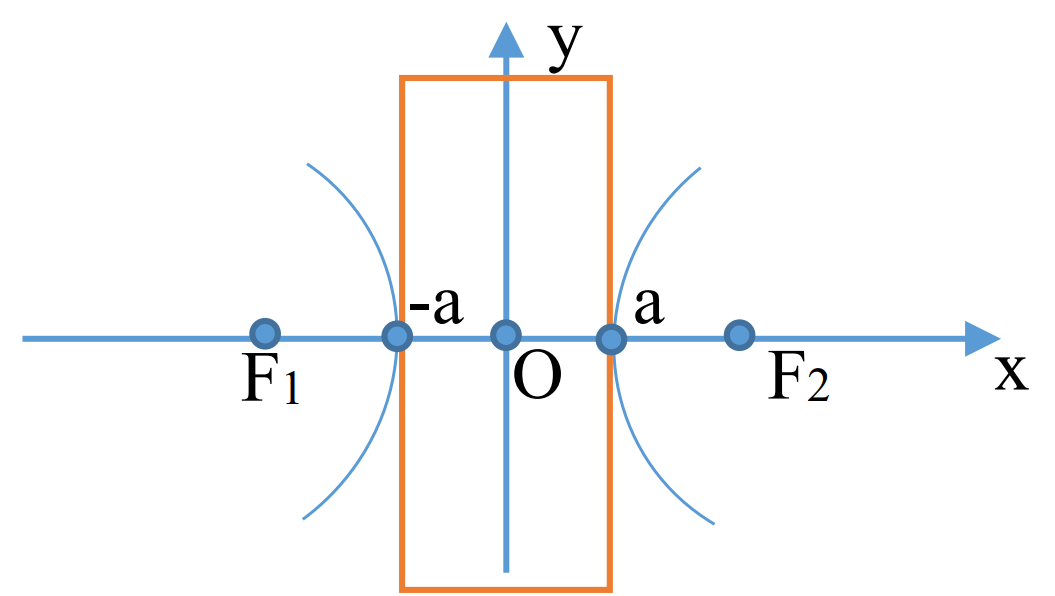
\includegraphics[scale=0.4]{images/gip2.png}
\end{center}
Так как все степени четные, то гипербола симметрична относительно осей $Ox, Oy$ и точки $O(0, 0)$. \\\\
$\bullet$ \textit{Центр симметрии
	гиперболы (центр между $F_1$ и $F_2$) называется \textbf{центром гиперболы}. Ось симметрии, проходящая
	через фокусы, называется \textbf{действительной (фокальной) осью}, а перпендикулярная ей ось,
	проходящая через центр гиперболы --- \textbf{мнимой осью}. Точки пересечения гиперболы с действительной
	осью являются её \textbf{вершинами}. Величины $a, b$ называются соответственно \textbf{действительными и
		мнимыми полуосями}. Если $a = b$, то гиперболу называют \textbf{равносторонней}.}\\\\
Исследуем формулу гиперболы в первой четверти, выразив $y$ из канонического уравнения:\\
$y= \dfrac{b}{a}(x^2 - a^2)^{\frac{1}{2}}$. \\$y' = \dfrac{1}{a}\cdot x(x^2 - a^2)^{\dfrac{1}{2}} > 0$, то есть функция возрастает;\\
$y'' = \dfrac{1}{a}(x^2 - a^2)^{-\frac{3}{2}}(-a^2) < 0$, то есть график функции вогнут.\\\\
Асимптота гиперболы в 1-й четверти: $y = kx + l$.\\ $k = \lim\limits_{x \to \infty}\dfrac{y}{x} = \lim\limits_{x \to \infty} \dfrac{b}{a}\cdot \dfrac{\sqrt{x^2 - a^2}}{x} = \dfrac{b}{a};\\ l = \lim\limits_{x \to \infty}x\dfrac{b}{a}y = 0 \Rightarrow y = \dfrac{b}{a}x$.

\section{Эксцентриситет и директрисы эллипса и гиперболы.}
Рассмотрим эллипс, у которого фокусное расстояние равно $2c$, а сумма расстояний от точек эллипса до фокусов $2a$. Тогда каноническое уравнение эллипса имеет вид $\dfrac{x_1^2}{a^2} + \dfrac{y_1^2}{b^2} = 1$, где $b^2 = a^2 - c^2$.\\\\
Рассмотрим гиперболу, у которой фокусное расстояние равно $2c$, а модуль разности расстояний от
точек гиперболы до фокусов $2a$. Тогда каноническое уравнение гиперболы имеет вид $\dfrac{x_1^2}{a^2} - \dfrac{y_1^2}{b^2} = 1$, где $b^2 = c^2 - a^2$.\\\\
$\bullet$ \textit{\textbf{Эксцентриситетом эллипса (гиперболы)} называется величина, равная $\upvarepsilon = \dfrac{c}{a}$.}\\\\
Заметим, что для эллипса $a > c \Rightarrow 0 < \upvarepsilon < 1$, для гиперболы $a < c \Rightarrow \upvarepsilon > 1.$\\\\
$\bullet$ \textit{Прямые $\Delta_1$ и $\Delta_2$, проходящие перпендикулярно фокальной оси эллипса (гиперболы) на
	расстоянии равном $\dfrac{a}{\upvarepsilon}$ от центра эллипса (гиперболы), называются \textbf{директрисами эллипса (гиперболы)}.}\\\\
Если эллипс и гипербола заданы каноническим уравнением, то уравнение директрисы имеет вид $x = \pm \frac{a}{\upvarepsilon}$.\\\\
Директрисы расположены по разные стороны от $Oy$. Фокус и директриса, расположенные по одну
сторону от $Oy$, называются \textbf{соответствующими друг другу}.\\
\begin{center}
	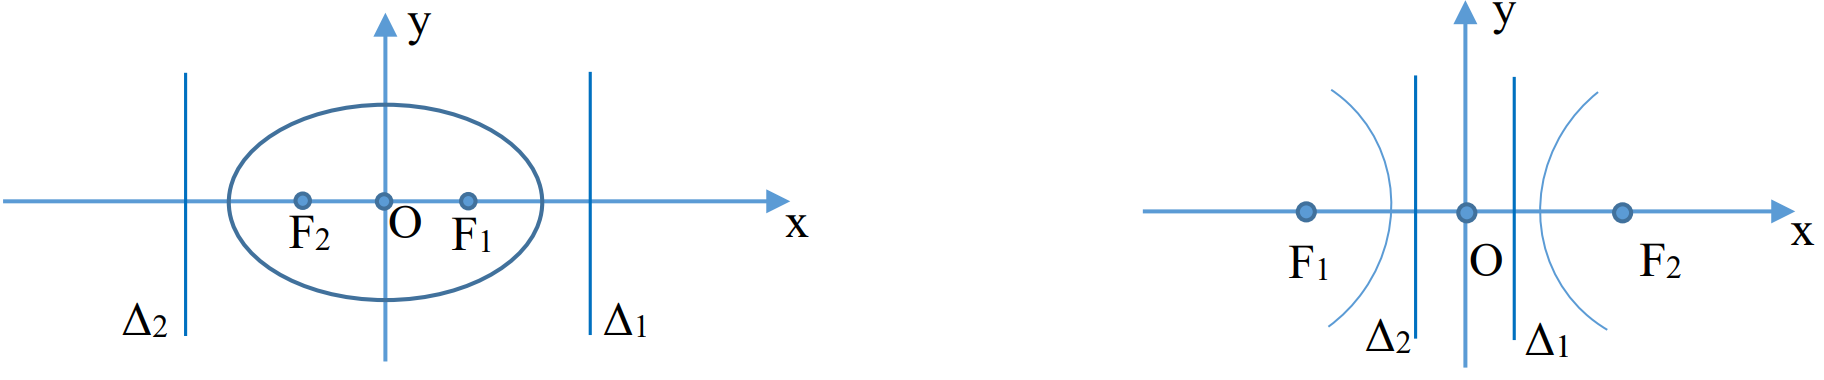
\includegraphics[scale=0.5]{images/exc1.png}
\end{center}
\newtheorem*{t3_1}{Теорема (основное свойство директрисы)}
\begin{t3_1}
	Отношение расстояния от произвольной точки эллипса
	(гиперболы) до фокуса $F_i$ к расстоянию этой точки до соответствующей этому фокусу директрисы
	равна эксцентриситету эллипса (гиперболы). То есть $$\dfrac{p(M_0,F_i)}{p(M_0,\Delta_i)} = \upvarepsilon.$$
\end{t3_1}
\begin{Proof}
	Пусть точка $M_0(x_0, y_0)$ принадлежит эллипсу $\dfrac{x_1^2}{a^2} + \dfrac{y_1^2}{b^2} = 1$. Тогда $|\overline{M_0F_1}| = |a - \dfrac{c}{a}x_0| = |a - \upvarepsilon x_0|$ и $|\overline{M_0F_2}| = |a + \upvarepsilon x_0|$. Следовательно, так как $\Delta_1 = x + \dfrac{a}{\upvarepsilon},\ \Delta_2 = -x - \dfrac{a}{\upvarepsilon}$, то $\rho (M_0, \Delta_1) = |x_0 -\dfrac{a}{\upvarepsilon}|,\ \rho(M_0,\Delta_2) = |x_0 +\dfrac{a}{\upvarepsilon}|$. Получаем $\dfrac{\rho(M_0, F_i)}{\rho(M_0, \Delta_i)} = \dfrac{|a-\upvarepsilon x_0|}{|x_0 - \frac{a}{\upvarepsilon}|} =\dfrac{|a-\upvarepsilon x_0|}{|\frac{a - \upvarepsilon x_0}{\upvarepsilon}|} = |\upvarepsilon| = \upvarepsilon$. Аналогично и во втором случае и для гиперболы.
\end{Proof}
\newtheorem*{th3_1_2}{Теорема}\begin{th3_1_2}
	Пусть в плоскости задана некоторая прямая $\Delta$ и точка $F$, не лежащая на ней. Множество
	точек плоскости, для которых отношение $\mu$ равняется отношению расстояния до $F$ к расстоянию до $\Delta$
	и отлично от 1, является эллипсом, если $\mu < 1$, и гиперболой, если $\mu > 1$. При этом точка $F$ будет
	являться фокусом, $\Delta$ --- директрисой, а $\mu$ --- эксцентриситетом.
\end{th3_1_2}
\begin{Proof}
	Построим ДПСК так, чтобы $Oy$
	совпадала с $\Delta$, а $Ox$ проходила через $F$.
	\begin{center}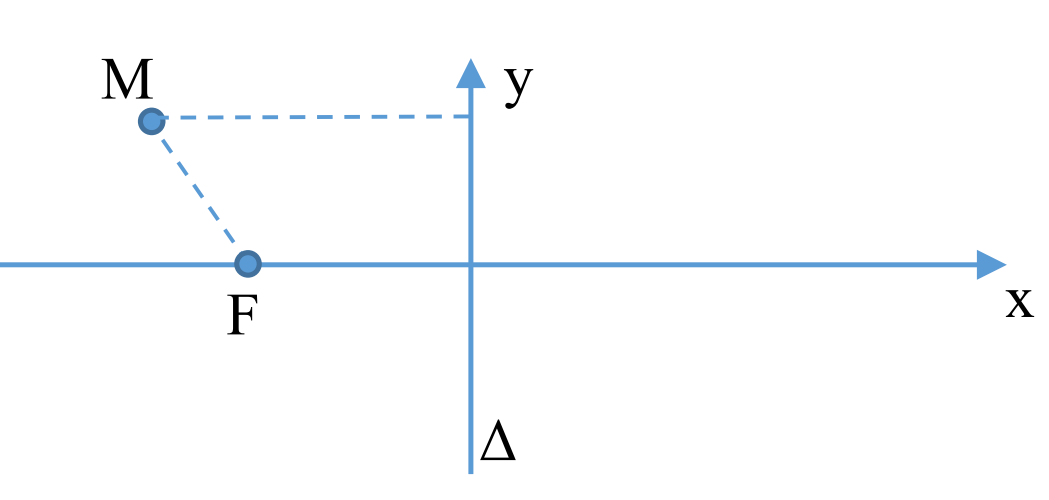
\includegraphics[scale=0.4]{images/exc2.png}\end{center}
	Точка $F$ будет иметь координаты $(k, 0)$, а $p(F, \Delta) = |k|$.\\\\
	Пусть $M(x, y)$ --- некоторая точка, удовлетворяющая
	отношению: $\mu = \dfrac{p(M,F)}{p(M,\Delta)}$. Преобразуем данное неравенство:
	$\dfrac{\sqrt{(x-k)^2+y^2}}{|x|} = \mu \Rightarrow \sqrt{(x-k)^2 + y^2} = \mu |x| \Rightarrow$ (возведём в квадрат и раскроем скобки) $x^2 + k^2 - 2kx + y^2 = \mu^2 x^2 \Rightarrow x^2(1 - \mu^2) + k^2 - 2kx + y^2 = 0 \Rightarrow
	x^2(1 - \mu^2) - 2kx + y^2 = -k^2 \Rightarrow$ (добавим в обе части неравенства выражение $\frac{k^2}{1-\mu^2}$)\\
	$x^2(1-\mu^2) - 2kx + \dfrac{k^2}{1-\mu^2} + y^2 = \dfrac{k^2}{1-u^2} - k^2 \Rightarrow$ (в левой части во всех слагаемых, за исключением $y^2$, выносим за скобки $(1-\mu^2))$\\
	$(1-\mu^2)(x^2 - \dfrac{2kx}{1-\mu^2} + \dfrac{k^2}{(1-\mu^2)^2}) + y^2 = \dfrac{k^2}{1-\mu^2} - k^2 \Rightarrow$ (слева получился квадрат разности, а справа приведём к общему знаменателю)\\
	$(1-\mu^2)(x^2 - \dfrac{k}{1-\mu^2})^2 + y^2 = \dfrac{k^2\mu^2}{1-\mu^2} \Rightarrow $ (поделим обе части на $1-\mu^2$)\\
	$(x^2- \dfrac{k}{1-\mu^2})^2 + \dfrac{y^2}{1-\mu^2} = \dfrac{k^2\mu^2}{(1-\mu^2)^2}.$\\\\
	Выполним замену $a = |\dfrac{k\mu}{1-\mu^2}|$ и выполним преобразование параллельного переноса ДПСК:\\
	$$\begin{cases}
		x'= x - \dfrac{k}{1-\mu^2},\\
		y' = y.
	\end{cases}$$
	Тогда, поделив на правую часть, получим $$\dfrac{(x')^2}{a^2} + \dfrac{(y')^2}{a^2(1-\mu^2)} = 1.\eqno (5.3.1)$$ Если $\mu < 1$, то уравнение (5.3.1) является каноническим уравнением эллипса, а если $\mu > 1$ --- гиперболы.\\\\
	Покажем, что $\mu$ --- эксцентриситет. Если уравнение (5.3.1) задает эллипс, то $\upvarepsilon = \dfrac{c}{a} = [b^2 = a^2 -c^2 \Rightarrow c^2 = a^2 - b^2] = \dfrac{\sqrt{a^2-b^2}}{a} = [b^2 = a^2(1-\mu^2)$ из (1)$] = \dfrac{\sqrt{a^2-a^2(1-\mu^2)}}{a} = \mu$. Если гипербола, то $b^2 = c^2 - a^2 \Rightarrow c^2 = a^2 + b^2$ и аналогично.\\\\
	$x' = \pm \dfrac{a}{\upvarepsilon} \Rightarrow x = \pm \dfrac{a}{\upvarepsilon} + \dfrac{k}{1-\mu^2} = \pm \dfrac{|\frac{k\mu}{1-\mu^2}|}{\upvarepsilon} + \dfrac{k}{1-\mu^2} \Rightarrow$ одно из уравнений имеет вид $x = 0$. В ДПСК $O’x’y’$ точка $F$ будет иметь координаты $(\pm c, 0)$, директрисы будут иметь уравнение $\pm \dfrac{a}{\upvarepsilon} \Rightarrow$ выполнив обратный перенос ДПСК получим, что одна из директрис совпадает с прямой $\Delta$ и один из фокусов совпадает с точкой $F$.
\end{Proof}\\\\
После доказательства теоремы определения эллипса и гиперболы можно дать по-новому.\\\\
$\bullet$ \textit{\textbf{Эллипсом (гиперболой)} называется множество точек на плоскости, для которых
	отношения расстояния до заданной точки, называемой \textbf{фокусом}, к расстоянию до
	заданной прямой, называемой \textbf{директрисой}, постоянно меньше единицы (больше
	единицы).}


\section{Парабола.}
$\bullet$ \textit{\textbf{Параболой} называется множество точек плоскости, каждая из которых равноудалена от точки называемой \textbf{фокусом} и от прямой называемой \textbf{директрисой}.}\\\\
Выведем уравнение параболы. Построим ДПСК так, чтобы ось $Ox$ проходила через фокус $F$ перпендикулярно прямой $\Delta$. И пусть $D$ --- точка пересечения прямой $\Delta$ и оси $Ox$. Направление $Ox$ выберем так, чтобы оно совпадало с направлением вектора $\overrightarrow{DF}$. Начало координат будет располагаться в центре между точками $D$ и $F$. \begin{center}
	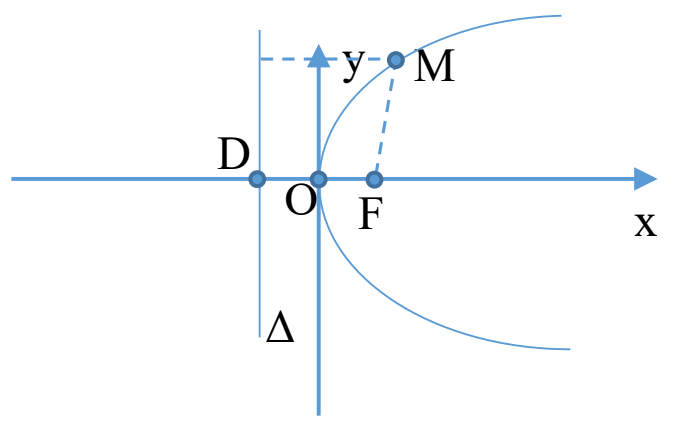
\includegraphics[scale=0.3]{images/parab.png}
\end{center} Обозначим за $p$ расстояние $\rho(F, \Delta)$. Тогда точка $F$ будет иметь координаты $(\frac{p}{2}, 0)$ и координата $x$ точки $D$ равна $-\frac{p}{2}$. Следовательно, получим $$x + \frac{p}{2} = 0\quad (x - \frac{p}{2} = 0).\eqno(5.4.1)$$
$\bullet$ \textit{Уравнение $(5.4.1)$ называется \textbf{нормальным уравнением параболы}.}\\\\
Пусть $M(x,y)$ --- произвольная точка параболы. Тогда $\rho(M, F) = \rho(M,\Delta)\Rightarrow\sqrt{(x-\frac{p}{2})^2 + y^2} = |-x-\frac{p}{2}|$. Возведем в квадрат, раскроем скобки и получим $x^2 + \frac{p^2}{2} - px + y^2 = x^2 \frac{p^2}{2} + px \Rightarrow$ $$y^2 = 2px.\eqno(5.4.2)$$
$\bullet$ \textit{Уравнение $(5.4.2)$ называется \textbf{каноническим уравнением параболы}. При этом параметр $p$ называется \textbf{фокальным} параметром.}\\\\
Исследование формы параболы по её каноническому уравнению:\\\\
Пусть $x \geqslant 0$. Тогда парабола находится в I и IV четвертях. Так как уравнение содержит $y$ в чётной степени, то парабола симметрична относительно оси $Ox$.\\\\
$\bullet$ \textit{Ось симметрии называется \textbf{осью} параболы. Точка $O(0,0)$ пересечения оси параболы и самой параболы называется \textbf{вершиной} параболы}.\\\\
Рассмотрим поведение параболы в I четверти, то есть при $x > 0, y> 0$:\\
$y = \sqrt{2px}$. Тогда $y' = \dfrac{\sqrt{2p}}{2}x^{-\frac{1}{2}}>0$, то есть функция возрастает. И $y'' = -\dfrac{\sqrt{2p}}{4}x^{-\frac{3}{2}}<0$, то есть функция выпукла. Асимптот нет, так как $k = \lim\limits_{x\to\infty} \dfrac{\sqrt{2px}}{x} = 0$, а $b = \infty$.

\section{Линии второго порядка.}
$\bullet$ \textit{\textbf{Алгебраической линией второго порядка} называется множество точек плоскости,
	координаты которых удовлетворяют уравнению $$Ax^2 + 2Bxy + Cy^2 + 2Dx + 2Ey + F = 0,\eqno(5.5.1)$$ где коэффициенты $A, B$ и $C$ не обращаются в нуль одновременно. В случае, если уравнению $(5.5.1)$ не удовлетворяет ни одна из точек, то это уравнение определяет \textbf{мнимую линию}.}\\\\
Определим, какие линии будут являться линиями второго порядка.\\
Пусть $B \ne 0$. Построим ДПСК $O'x'y'$, которая получена из ДПСК $Oxy$ поворотом против часовой стрелки вокруг начала координат на угол $\varphi$. Тогда $\begin{cases}
	x = x' cos\varphi - y' sin\varphi,\\
	y = x'sin\varphi + y'cos\varphi.
\end{cases}$.\\ Заменим и получим $A(x'cos\varphi - y' sin\varphi)^2 + 2B(x'cos\varphi - y'sin\varphi)\cdot (x'cos\varphi + y'sin\varphi) + C(x'cos\varphi + y' sin\varphi)^2 + 2D(x'cos\varphi - y' sin \varphi) + 2E(x'cos\varphi + y' sin\varphi) + F = 0$.\\
Ракскрыв скобки и приведя подобные, получим $$A'(x')^2 + 2Bx'y' + C'(y')^2 + 2D'x' + 2E'y' + F = 0.\eqno(5.5.2)$$
Покажем, что коэффициенты $A'$, $B'$ и $C'$ не обращаются одновременно в нуль:\\
$A' = A\cdot cos^2\varphi + 2B\cdot cos\varphi\cdot sin\varphi + C\cdot sin^2\varphi;$\\
$B' = -A\cdot cos\varphi\cdot sin\varphi + B\cdot (cos^2\varphi - sin^2\varphi) + C\cdot sin\varphi\cdot cos\varphi;$\\
$C' = A\cdot sin^2\varphi - 2B\cdot cos\varphi\cdot sin\varphi + C\cdot cos^2 \varphi.$\\
Предположим, что $A'$, $B'$ и $C'$ равны нулю. Сложив первое и третье уравнения, получим $A + C = 0$. Следовательно, $C = -A$. Из второго уравнения, приведя по формуле синуса и косинуса двойного угла, получим $0 = -A\cdot sin(2\varphi) + B\cdot cos(2\varphi)$, а из первого уравнения этой же заменой получим $0 = A\cdot cos(2\varphi) + B\cdot sin (2\varphi)$. Следовательно, получим систему
$$\begin{cases}
	A\cdot cos (2\varphi) + B\cdot sin (2\varphi) = 0,\\
	-A\cdot sin(2\varphi) + B\cdot cos (2\varphi) = 0.
\end{cases}$$
Определитель матрицы системы равен 1. В таком случае система будет иметь единственное решение $A = B = 0 = C$, что является противоречием с тем, что уравнение (5.5.1) --- уравнение линии второго порядка. Значит коэффициенты $A'$, $B'$ и $C'$ не обращаются в нуль одновременно.\\\\
Подберем угол $\varphi$ так, чтобы коэффициент $B'$ стал равен нулю. То есть $-A\cdot cos\varphi \cdot sin\varphi + B(cos^2\varphi - sin^2\varphi) + C\cdot sin\varphi \cdot cos\varphi = 0 \Leftrightarrow \dfrac{C - A}{2}\cdot sin(2\varphi) + B\cdot cos(2\varphi) = 0\Leftrightarrow \dfrac{A - C}{2}\cdot sin(2\varphi) = B\cdot cos(2\varphi)$. Если $A - C \ne 0$, то $tg(2\varphi) = \dfrac{2B}{A - C}$. Если же $A - C = 0$, то $B\ne 0$. Следовательно, $cos2(\varphi) = 0\Rightarrow 2\varphi = \dfrac{\pi}{2}\Rightarrow \varphi = \dfrac{\pi}{4}$.\\\\
В результате получим ДПСК, в которой уравнение линий второго порядка имеет вид $$A'(x')^2 + C'(y')^2 + 2D'x' + 2E'y' + F = 0.\eqno(5.5.3)$$
\begin{enumerate}
	\item Пусть коэффициенты $A'$ и $C'$ ненулевые. Преобразуем уравнение следующим образом: добавим и вычтем числа $\dfrac{(D')^2}{A'}$ и $\dfrac{(E')^2}{C'}$. Везде, где есть $x'$ или $D'$ вынесем коэффициент $A'$ за скобки. Аналогично, где $y'$ или $E'$ --- $C'$ за скобки. Обозначим за $F'$ выражение $F' = F - \dfrac{(D')^2}{A'} - \dfrac{(E')^2}{C'}$. В итоге получим $A'\Big((x')^2 + 2\dfrac{D'x'}{A'} + (\dfrac{D'}{A'})^2\Big) + C'\Big((y')^2 + 2\dfrac{E'y'}{C'}+(\dfrac{E'}{C'})^2\Big) + F' = 0 \Longleftrightarrow$ (свернем квадраты суммы) $A'(x' + \dfrac{D'}{A'})^2 + B'(y' + \dfrac{E'}{C'})^2 + F' =~ 0$. Выполним параллельный перенос ДПСК: $\begin{cases}
		x'' = x' + \dfrac{D'}{A'},\\
		y'' = y' + \dfrac{E'}{C'}.
	\end{cases}$ Отсюда получим $$A'(x'')^2 + C'(y'')^2 = -F'.\eqno(5.5.4)$$
	Здесь рассмотрим два случая:\begin{enumerate}
		\item Пусть $F' \ne 0$. Тогда поделим уравнение (5.5.4) на $-F'$, перенесем $A'$ и $C'$ в знаменатели и получим $\dfrac{(x'')^2}{\frac{-F}{A'}} + \dfrac{(y'')^2}{\frac{-F}{C'}} = 1$.\\
		Если знаменатели положительные, то уравнение примет вид $\dfrac{(x'')^2}{a^2} + \dfrac{(y'')^2}{b^2} = 1$, что является к\textbf{аноническим уравнением эллипса}.\\ Если знаменатели отрицательные, то уравнение примет вид $\dfrac{(x'')^2}{a^2} + \dfrac{(y'')^2}{b^2} = -1$, что является \textbf{каноническим уравнением мнимого эллипса}.
		\item Пусть $F' = 0$. Тогда поделим обе части уравнения (5.5.4) на $A'C'$ и получим уравнение $\dfrac{(x'')^2}{C'} + \dfrac{(y'')^2}{A'} = 0$. \\Если знаменатели разных знаков, то уравнение примет вид $\dfrac{(x'')^2}{a^2} - \dfrac{(y'')^2}{b^2} = 0$, что является \textbf{каноническим уравнением пары пересекающиъся прямых}. \\Если знаменатели имеют один знак, то уравнение примет вид $\dfrac{(x'')^2}{a^2} + \dfrac{(y'')^2}{b^2} = 0$, что является \textbf{каноническим уравнением пары мнимых пересекающихся прямых}. Заметим, что точка $(0,0)$ удовлетворяет этому уравнению.
	\end{enumerate}
	\item Пусть $A' \ne 0, C' = 0$ (аналогично будет и наоборот). Уравнение (5.5.3) примет вид $A'((x')^2+2\dfrac{D'x'}{A'} + (\dfrac{D'}{A'})^2) + 2E'y' + F - \dfrac{(D')^2}{A'} = 0$. Аналогично с пунктом 1 рассмотрим 2 случая: \begin{enumerate}
		\item Пусть $E' \ne 0$. Тогда вынесем во всех слагаемых, кроме тех, у которых есть множитель $A'$, за скобку $2E'$. Получим $$A'(x' + \dfrac{D'}{A'})^2 + 2E'(y' + \dfrac{F}{2E'} + \dfrac{(D')^2}{2E'A'}) = 0.\eqno(5.5.5)$$ Выполним преобразование симметрии и получим уравнение вида $(y'')^2 = 2px''$, что является \textbf{каноническим уравнением параболы}.
		\item Пусть $E'=0$. Тогда уравнение (5.5.5) примет вид $A'(x' + \dfrac{D'}{A'})^2 + F - \dfrac{(D')^2}{A'} = 0$. Выполним преобразование переноса $\begin{cases}
			x'' = x' + \dfrac{D'}{A'},\\
			y'' = y';
		\end{cases}$ и заменим $F - \dfrac{(D')^2}{A'}$ на $F''$. В результате этих действий получим $(x'')^2 + \dfrac{F''}{A'} = 0$. \\Если $\dfrac{F''}{A'} <0$, то $(x'')^2 - a^2 = 0$, что является \textbf{каноническим уравнением пары\\\\ параллельных прямых}. \\Если $\dfrac{F''}{A'} =0$, то $(x'')^2$, что является \textbf{каноническим уравнением пары\\\\ совпадающих прямых}. \\А если $\dfrac{F''}{A'} >0$, то $(x'')^2 + a^2 = 0$, что является \textbf{каноническим уравнением\\\\ пары мнимых параллельных прямых}.
	\end{enumerate}
\end{enumerate}
Таким образом нами была доказана следующая теорема.
\newtheorem*{th5_5}{Теорема}\begin{th5_5}Для любой линии второго порядка существует ДПСК, в которой данная линия задается одним из следующих канонических уравнений:
	\begin{enumerate}
		\item $\dfrac{x^2}{a^2} + \dfrac{y^2}{b^2} = 1$ --- эллипс;
		\item $\dfrac{x^2}{a^2} + \dfrac{y^2}{b^2} = -1$ --- мнимый эллипс;
		\item $\dfrac{x^2}{a^2} - \dfrac{y^2}{b^2} = 1$ --- гипербола;
		\item $\dfrac{x^2}{a^2} - \dfrac{y^2}{b^2} = 0$ --- пара пересекающихся прямых;
		\item $\dfrac{x^2}{a^2} + \dfrac{y^2}{b^2} = 0$ --- пара мнимых пересекающихся прямых;
		\item $y^2 = 2px$ --- парабола;
		\item $x^2 - a^2 = 0$ --- пара параллельных прямых;
		\item $x^2 + a^2 = 0$ --- пара мнимых параллельных прямых;
		\item $x^2 = 0$ --- пара совпадающих прямых.
	\end{enumerate}
\end{th5_5}

\section{Поверхности второго порядка.}

$\bullet$ \textit{\textbf{Поверхностью второго порядка} называется множество точек пространства, декартовые координаты которых удовлетворяют уравнению следующего вида: $$a_{11}x^2 + a_{22}y^2 + a_{33}z^2 + 2a_{12}xy + 2a_{13}xz + 2a_{23}yz + 2b_1x + 2b_2y + 2b_3z + c = 0.\eqno(5.6.1)$$}
Если уравнению (5.6.1) не удовлетворяет ни одна точка, то поверхность мнимая.
\newtheorem*{th21_1}{Теорема}\begin{th21_1}Для любой поверхности второго порядка существует пространтсвенная ДПСК в которой эта поверхность определена одним из следующих канонических уравнений:
	\begin{enumerate}
		\item $\dfrac{x^2}{a^2} + \dfrac{y^2}{b^2} + \dfrac{z^2}{c^2} = 1$ --- эллипсоид;
		\item $\dfrac{x^2}{a^2} + \dfrac{y^2}{b^2} + \dfrac{z^2}{c^2} = -1$ --- мнимый эллипсоид;
		\item $\dfrac{x^2}{a^2} + \dfrac{y^2}{b^2} - \dfrac{z^2}{c^2} = 1$ --- однополостной гиперболоид;
		\item $\dfrac{x^2}{a^2} + \dfrac{y^2}{b^2} - \dfrac{z^2}{c^2} = -1$ --- двуполостной гиперболоид;
		\item $\dfrac{x^2}{a^2} + \dfrac{y^2}{b^2} - \dfrac{z^2}{c^2} = 0$ --- конус второго порядка;
		\item $\dfrac{x^2}{a^2} + \dfrac{y^2}{b^2} + \dfrac{z^2}{c^2} = 0$ --- мнимый конус второго порядка;
		\item $\dfrac{x^2}{a^2} + \dfrac{y^2}{b^2} = 2z$ --- эллиптический параболоид;
		\item $\dfrac{x^2}{a^2} - \dfrac{y^2}{b^2} = 2z$ --- гиперболический параболоид;
		\item $\dfrac{x^2}{a^2} + \dfrac{y^2}{b^2} = 1$ --- эллиптический цилиндр;
		\item  $\dfrac{x^2}{a^2} + \dfrac{y^2}{b^2} = -1$ --- мнимый эллиптический цилиндр;
		\item $\dfrac{x^2}{a^2} - \dfrac{y^2}{b^2} = 1$ --- гиперболический цилиндр;
		\item $y^2 = 2px$ --- параболоический цилиндр;
		\item $\dfrac{x^2}{a^2} - \dfrac{y^2}{b^2} = 0$ --- пара пересекающихся плоскостей;
		\item $\dfrac{x^2}{a^2} + \dfrac{y^2}{b^2} = 0$ --- пара мнимых пересекающихся плоскостей;
		\item $x^2 - a^2 = 0$ --- пара параллельных плоскостей;
		\item $x^2 + a^2 = 0$ --- пара мнимых параллельных плоскостей;
		\item $x^2 = 0$ --- пара совпадающих плоскостей.
	\end{enumerate}
\end{th21_1}
\begin{center}  
	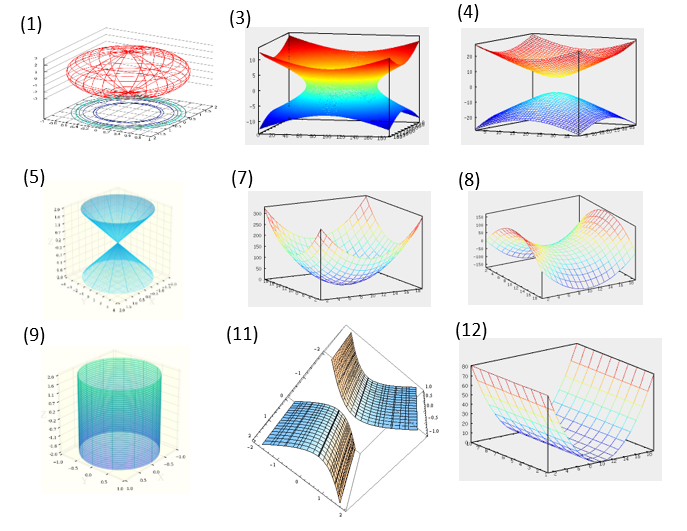
\includegraphics[width=1\textwidth]{images/П2П_1.PNG}
\end{center}




\section{Цилиндрические и конические поверхности. Линейчатые поверхности. Поверхности вращения.}
$\bullet$ \textit{\textbf{Цилиндрической поверхностью} называется объединение всех параллельных прямых, которые пересекают некоторую линию $L$, при этом линия $L$ называется \textbf{направляющей} цилиндрической поверхности, а прямые, из которых состоит поверхность, называются \textbf{образующими}}.\\\\
Пусть линия $L$ задается как линия пересечения двух плоскостей, тогда она определена системой двух уравнений $$\begin{cases}
	F_1(x,y,z) = 0,\\
	F_2(x,y,z) = 0.
\end{cases}$$ И пусть образующие цилиндрической поверхности имеют направляющий вектор $a(a_1, a_2, a_3)$. Точка $M(x,y,z)$ принадлежит цилиндрической поверхности $\Longleftrightarrow$ существует точка $M_0(x_0, y_0, z_0)$ такая, что\begin{enumerate}
	\item $M_0 \in L$;
	\item $\overline{M_0M} \parallel a.$
\end{enumerate}
Тогда получаем систему $$\begin{cases}
	F_1(x_0,y_0,z_0) = 0,\\
	F_2(x_0,y_0,z_0) = 0,\\
	\dfrac{x-x_0}{a_1} = \dfrac{y-y_0}{a_2} = \dfrac{z-z_0}{a_3}.
\end{cases}$$ Исключив из этой системы $x_0, y_0$ и $z_0$, получим \textbf{уравнение цилиндрической поверхности}.\\\\
$\bullet$ \textit{\textbf{Канонической поверхностью} называется объединение всех прямых, которые проходят через некоторую точку $P$ и пересекают некоторую линию $L$. При этом линия $L$ называется \textbf{направляющей} канонической поверхности, а точка $P$ --- \textbf{вершиной} канонической поверхности.}\\\\
Пусть точка $P$ имеет координаты $(x_1, y_1, z_1)$. Точка $M(x,y,z)$ принадлежит канонической поверхности $\Longleftrightarrow$ существует точка $M_0(x_0, y_0, z_0)$ такая, что\begin{enumerate}
	\item $M_0 \in L$;
	\item $\overline{PM} \parallel \overline{PM_0}.$
\end{enumerate}
Тогда получаем систему $$\begin{cases}
	F_1(x_0,y_0,z_0) = 0,\\
	F_2(x_0,y_0,z_0) = 0,\\
	\dfrac{x-x_1}{x_0-x_1} = \dfrac{y-y_1}{y_0 - y_1} = \dfrac{z-z_1}{z_0 - z_1}.
\end{cases}$$ Исключив из этой системы $x_0, y_0$ и $z_0$, получим \textbf{уравнение канонической повехности}.\\\\
$\bullet$ \textit{Поверхность называется \textbf{линейчатой}, если она образована движением прямой. При этом прямые, из которых состоит линейчатая поверхность, называются прямолинейными образующими.}\\\\
Цилиндрическая и каноническая поверхности являются линейчатыми поверхностями. \\\\Среди поверхностей второго порядка прямолинейными образующими обладают однополостный гиперболоид и гиперболический параболоид. Докажем это. Для этого рассмотрим однополостный гиперболоид. Тогда выполняется $\dfrac{x^2}{a^2} + \dfrac{y^2}{b^2} - \dfrac{z^2}{c^2} = 1$. Перенесем $\dfrac{y^2}{b^2}$ в правую часть и распишем разность квадратов: $\Big(\dfrac{x}{a} - \dfrac{z}{c}\Big)\Big(\dfrac{x}{a} + \dfrac{z}{c}\Big) = \Big(1 - \dfrac{y}{b}\Big)\Big(1 + \dfrac{y}{b}\Big).$ Составим систему. При фиксированных $k$ эта система определяет прямую. Причем если точка $M$ лежит на этой прямой, то она лежит и на однополостном гиперболоиде. Следовательно, все прямые целиком лежат на однополостном гиперболоиде. $$\begin{cases}
	\dfrac{x}{a} - \dfrac{z}{c} = \Big(1-\dfrac{y}{b}\Big) \cdot k,\\\\
	\dfrac{x}{a} + \dfrac{z}{c} = \Big(1+\dfrac{y}{b}\Big) \cdot \dfrac{1}{k};
\end{cases}, k \in \mathbb{R}.\eqno(5.7.1)$$
Покажем обратное. Пусть $M_0(x_0, y_0, z_0)$ --- произвольная точка однополостного гиперболоида. Тогда  $\dfrac{x_0^2}{a^2} + \dfrac{y_0^2}{b^2} - \dfrac{z_0^2}{c^2} = 1$. Найдем $k_0$ из уравнений: $$\begin{cases}
	\dfrac{x_0}{a} - \dfrac{z_0}{c} = \Big(1-\dfrac{y_0}{b}\Big) \cdot k,\\\\
	\dfrac{x_0}{a} + \dfrac{z_0}{c} = \Big(1+\dfrac{y_0}{b}\Big) \cdot \dfrac{1}{k}.
\end{cases}$$ Следовательно, точка $M_0$ лежит на прямой (5.7.1). Аналогично монжо показать, что однополостный гиперболоид покрывается еще одним семейством прямых:  $$\begin{cases}
	\dfrac{x}{a} - \dfrac{z}{c} = \Big(1+\dfrac{y}{b}\Big) \cdot k,\\\\
	\dfrac{x}{a} + \dfrac{z}{c} = \Big(1-\dfrac{y}{b}\Big) \cdot \dfrac{1}{k}.
\end{cases}$$
Аналогично можно показать, что гиперболический параболоид также покрыт двумя семействами прямолинейных образующих. Для него выполняется $\dfrac{x^2}{a^2} - \dfrac{y^2}{b^2} = 2z$. Распишем разность квадратов и получим $\Big(\dfrac{x}{a}-\dfrac{y}{b}\Big)\Big(\dfrac{x}{a}+\dfrac{y}{b}\Big) = 2z$. Тогда\begin{center}
	$\begin{cases}
		\dfrac{x}{a} - \dfrac{y}{b} = 2kz,\\\\
		\dfrac{x}{a} + \dfrac{y}{b} = \dfrac{1}{k};
	\end{cases}$ --- первое семейство;\quad $\begin{cases}
		\dfrac{x}{a} - \dfrac{y}{b} = \dfrac{1}{k},\\\\
		\dfrac{x}{a} + \dfrac{y}{b} = 2kz;
	\end{cases}$ --- второе семейство;
\end{center}
$\bullet$ \textit{\textbf{Поверхностью вращения} линии $L$ вокруг прямой $\Delta$ называется объединение окружностей, которые}\begin{enumerate}
	\item \textit{пересекают линию $L$};
	\item \textit{имеют центры на прямой $\Delta$};
	\item \textit{лежат в плоскости, перпендикулярной $\Delta$}.
\end{enumerate}
Рассмотрим поверхность вращения линии $L$  такой, что $\begin{cases}
	F_1(x,y,z) = 0,\\
	F_2(x,y,z) = 0;
\end{cases}$ вокруг прямой $\Delta$ такой, что $\dfrac{x-x_1}{a_1} = \dfrac{y-y_1}{a_2} = \dfrac{z-z_1}{a_3}.$ Точка $M$ принадлежит поверхности вращения $\Longleftrightarrow$ существует точка $M_0(x_0, y_0, z_0)$ такая, что\begin{enumerate}
	\item $M_0\in L$;
	\item $\overrightarrow{M_0M}\perp a(a_1, a_2, a_3)$;
	\item $\rho(M_0, \Delta) = \rho (M,\Delta)$.
\end{enumerate} Тогда получаем систему $$\begin{cases}
	F_1(x_0,y_0,z_0) = 0,\\
	F_2(x_0,y_0,z_0) = 0,\\
	a_1\cdot(x-x_0) + a_2\cdot(y-y_0) + a_3\cdot (z-z_0) = 0,\\
	\rho(M_0, \Delta) = \rho (M,\Delta).
\end{cases}$$ Исключив из этой системы $x_0, y_0$ и $z_0$, получим \textbf{уравнение поверхности вращения}.